% Options for packages loaded elsewhere
\PassOptionsToPackage{unicode}{hyperref}
\PassOptionsToPackage{hyphens}{url}
\PassOptionsToPackage{dvipsnames,svgnames,x11names}{xcolor}
%
\documentclass[
  letterpaper,
  DIV=11,
  numbers=noendperiod]{scrartcl}

\usepackage{amsmath,amssymb}
\usepackage{iftex}
\ifPDFTeX
  \usepackage[T1]{fontenc}
  \usepackage[utf8]{inputenc}
  \usepackage{textcomp} % provide euro and other symbols
\else % if luatex or xetex
  \usepackage{unicode-math}
  \defaultfontfeatures{Scale=MatchLowercase}
  \defaultfontfeatures[\rmfamily]{Ligatures=TeX,Scale=1}
\fi
\usepackage{lmodern}
\ifPDFTeX\else  
    % xetex/luatex font selection
\fi
% Use upquote if available, for straight quotes in verbatim environments
\IfFileExists{upquote.sty}{\usepackage{upquote}}{}
\IfFileExists{microtype.sty}{% use microtype if available
  \usepackage[]{microtype}
  \UseMicrotypeSet[protrusion]{basicmath} % disable protrusion for tt fonts
}{}
\makeatletter
\@ifundefined{KOMAClassName}{% if non-KOMA class
  \IfFileExists{parskip.sty}{%
    \usepackage{parskip}
  }{% else
    \setlength{\parindent}{0pt}
    \setlength{\parskip}{6pt plus 2pt minus 1pt}}
}{% if KOMA class
  \KOMAoptions{parskip=half}}
\makeatother
\usepackage{xcolor}
\setlength{\emergencystretch}{3em} % prevent overfull lines
\setcounter{secnumdepth}{-\maxdimen} % remove section numbering
% Make \paragraph and \subparagraph free-standing
\ifx\paragraph\undefined\else
  \let\oldparagraph\paragraph
  \renewcommand{\paragraph}[1]{\oldparagraph{#1}\mbox{}}
\fi
\ifx\subparagraph\undefined\else
  \let\oldsubparagraph\subparagraph
  \renewcommand{\subparagraph}[1]{\oldsubparagraph{#1}\mbox{}}
\fi


\providecommand{\tightlist}{%
  \setlength{\itemsep}{0pt}\setlength{\parskip}{0pt}}\usepackage{longtable,booktabs,array}
\usepackage{calc} % for calculating minipage widths
% Correct order of tables after \paragraph or \subparagraph
\usepackage{etoolbox}
\makeatletter
\patchcmd\longtable{\par}{\if@noskipsec\mbox{}\fi\par}{}{}
\makeatother
% Allow footnotes in longtable head/foot
\IfFileExists{footnotehyper.sty}{\usepackage{footnotehyper}}{\usepackage{footnote}}
\makesavenoteenv{longtable}
\usepackage{graphicx}
\makeatletter
\def\maxwidth{\ifdim\Gin@nat@width>\linewidth\linewidth\else\Gin@nat@width\fi}
\def\maxheight{\ifdim\Gin@nat@height>\textheight\textheight\else\Gin@nat@height\fi}
\makeatother
% Scale images if necessary, so that they will not overflow the page
% margins by default, and it is still possible to overwrite the defaults
% using explicit options in \includegraphics[width, height, ...]{}
\setkeys{Gin}{width=\maxwidth,height=\maxheight,keepaspectratio}
% Set default figure placement to htbp
\makeatletter
\def\fps@figure{htbp}
\makeatother

% load packages
\usepackage{geometry}
\usepackage{xcolor}
\usepackage{eso-pic}
\usepackage{fancyhdr}
\usepackage{sectsty}
\usepackage{fontspec}
\usepackage{titlesec}

%% Set page size with a wider right margin
\geometry{a4paper, total={170mm,257mm}, left=20mm, top=20mm, bottom=20mm, right=50mm}

%% Let's define some colours
\definecolor{light}{HTML}{E6E6FA}
\definecolor{highlight}{HTML}{800080}
\definecolor{dark}{HTML}{330033}

%% Let's add the border on the right hand side 
\AddToShipoutPicture{% 
    \AtPageLowerLeft{% 
        \put(\LenToUnit{\dimexpr\paperwidth-3cm},0){% 
            \color{light}\rule{3cm}{\LenToUnit\paperheight}%
          }%
     }%
     % logo
    \AtPageLowerLeft{% start the bar at the bottom right of the page
        \put(\LenToUnit{\dimexpr\paperwidth-2.25cm},27.2cm){% move it to the top right
            \color{light}
\includegraphics[width=1.5cm]{_extensions/nrennie/PrettyPDF/logo.png}
          }%
     }%
}

%% Style the page number
\fancypagestyle{mystyle}{
  \fancyhf{}
  \renewcommand\headrulewidth{0pt}
  \fancyfoot[R]{\thepage}
  \fancyfootoffset{3.5cm}
}
\setlength{\footskip}{20pt}

%% style the chapter/section fonts
\chapterfont{\color{dark}\fontsize{20}{16.8}\selectfont}
\sectionfont{\color{dark}\fontsize{20}{16.8}\selectfont}
\subsectionfont{\color{dark}\fontsize{14}{16.8}\selectfont}
\titleformat{\subsection}
  {\sffamily\Large\bfseries}{\thesection}{1em}{}[{\titlerule[0.8pt]}]
  
% left align title
\makeatletter
\renewcommand{\maketitle}{\bgroup\setlength{\parindent}{0pt}
\begin{flushleft}
  {\sffamily\huge\textbf{\MakeUppercase{\@title}}} \vspace{0.3cm} \newline
  {\Large {\@subtitle}} \newline
  \@author
\end{flushleft}\egroup
}
\makeatother

%% Use some custom fonts
\setsansfont{Ubuntu}[
    Path=_extensions/nrennie/PrettyPDF/Ubuntu/,
    Scale=0.9,
    Extension = .ttf,
    UprightFont=*-Regular,
    BoldFont=*-Bold,
    ItalicFont=*-Italic,
    ]

\setmainfont{Ubuntu}[
    Path=_extensions/nrennie/PrettyPDF/Ubuntu/,
    Scale=0.9,
    Extension = .ttf,
    UprightFont=*-Regular,
    BoldFont=*-Bold,
    ItalicFont=*-Italic,
    ]
\KOMAoption{captions}{tableheading}
\makeatletter
\makeatother
\makeatletter
\makeatother
\makeatletter
\@ifpackageloaded{caption}{}{\usepackage{caption}}
\AtBeginDocument{%
\ifdefined\contentsname
  \renewcommand*\contentsname{Table of contents}
\else
  \newcommand\contentsname{Table of contents}
\fi
\ifdefined\listfigurename
  \renewcommand*\listfigurename{List of Figures}
\else
  \newcommand\listfigurename{List of Figures}
\fi
\ifdefined\listtablename
  \renewcommand*\listtablename{List of Tables}
\else
  \newcommand\listtablename{List of Tables}
\fi
\ifdefined\figurename
  \renewcommand*\figurename{Figure}
\else
  \newcommand\figurename{Figure}
\fi
\ifdefined\tablename
  \renewcommand*\tablename{Table}
\else
  \newcommand\tablename{Table}
\fi
}
\@ifpackageloaded{float}{}{\usepackage{float}}
\floatstyle{ruled}
\@ifundefined{c@chapter}{\newfloat{codelisting}{h}{lop}}{\newfloat{codelisting}{h}{lop}[chapter]}
\floatname{codelisting}{Listing}
\newcommand*\listoflistings{\listof{codelisting}{List of Listings}}
\makeatother
\makeatletter
\@ifpackageloaded{caption}{}{\usepackage{caption}}
\@ifpackageloaded{subcaption}{}{\usepackage{subcaption}}
\makeatother
\makeatletter
\@ifpackageloaded{tcolorbox}{}{\usepackage[skins,breakable]{tcolorbox}}
\makeatother
\makeatletter
\@ifundefined{shadecolor}{\definecolor{shadecolor}{rgb}{.97, .97, .97}}
\makeatother
\makeatletter
\@ifundefined{codebgcolor}{\definecolor{codebgcolor}{named}{light}}
\makeatother
\makeatletter
\makeatother
\ifLuaTeX
  \usepackage{selnolig}  % disable illegal ligatures
\fi
\IfFileExists{bookmark.sty}{\usepackage{bookmark}}{\usepackage{hyperref}}
\IfFileExists{xurl.sty}{\usepackage{xurl}}{} % add URL line breaks if available
\urlstyle{same} % disable monospaced font for URLs
\hypersetup{
  pdftitle={Information Systems Research Report},
  pdfauthor={S Bisetty (2874956), FJ Van Wyk (24880159), C Twaddle (23560444)},
  colorlinks=true,
  linkcolor={highlight},
  filecolor={Maroon},
  citecolor={Blue},
  urlcolor={highlight},
  pdfcreator={LaTeX via pandoc}}

\title{Information Systems Research Report}
\author{S Bisetty (2874956), FJ Van Wyk (24880159), C Twaddle
(23560444)}
\date{}

\begin{document}
\maketitle
\pagestyle{mystyle}

\ifdefined\Shaded\renewenvironment{Shaded}{\begin{tcolorbox}[boxrule=0pt, enhanced, breakable, borderline west={3pt}{0pt}{shadecolor}, frame hidden, sharp corners, colback={codebgcolor}]}{\end{tcolorbox}}\fi

\hypertarget{introduction}{%
\subsection{\texorpdfstring{\textbf{Introduction}}{Introduction}}\label{introduction}}

Information System (IS) research landscape has evolved and changed over
the past decade. This evolution is apparent in the shifting themes and
topics that were the focus of research. ~By utilising text-based
techniques, we uncovered prevalent trends, recurring themes and topic
relationships within IS literature.

\newpage{}

\hypertarget{most-common-topics-and-themes-in-is-research-2011-2020}{%
\subsection{\texorpdfstring{\textbf{1. Most Common Topics and Themes in
IS Research
(2011-2020)}}{1. Most Common Topics and Themes in IS Research (2011-2020)}}\label{most-common-topics-and-themes-in-is-research-2011-2020}}

Our analysis centred on a dataset comprising information on a variety of
IS research articles, such as the title, abstract, authors, year of
publication and keywords, that have been published over the past decade.
To ensure meaningful insights were extracted, the textual data had been
pre-processed to eliminate noise and retain only relevant information.
After which a Latent Dirichlet Allocation (LDA) model, a topic modelling
algorithm, was applied to identify the most common themes and topics
embedded within the corpus.

The K Value was calculated and selected after generating the following
graph that finds the topic number:

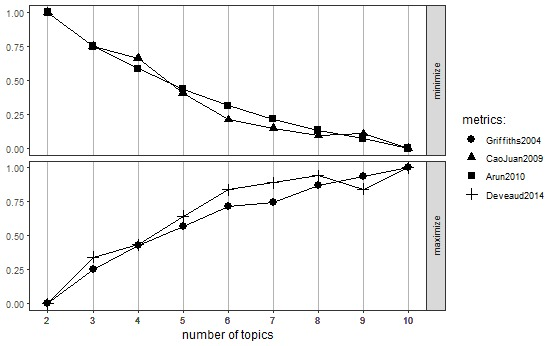
\includegraphics[width=5.20833in,height=\textheight]{images/FindTopicNumbers-01.jpg}

Applying LDA revealed ten distinct topics that are characterised by a
set of keywords that represent the focal points of discussion. These
keywords can be found below:

Results:

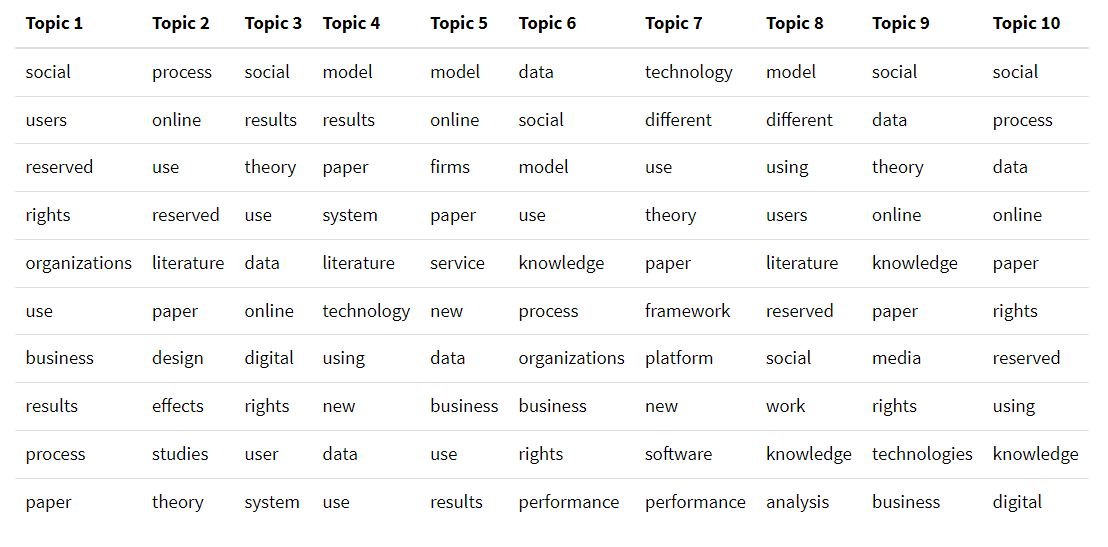
\includegraphics[width=5.20833in,height=\textheight]{images/TopicLDAResults-01.png}

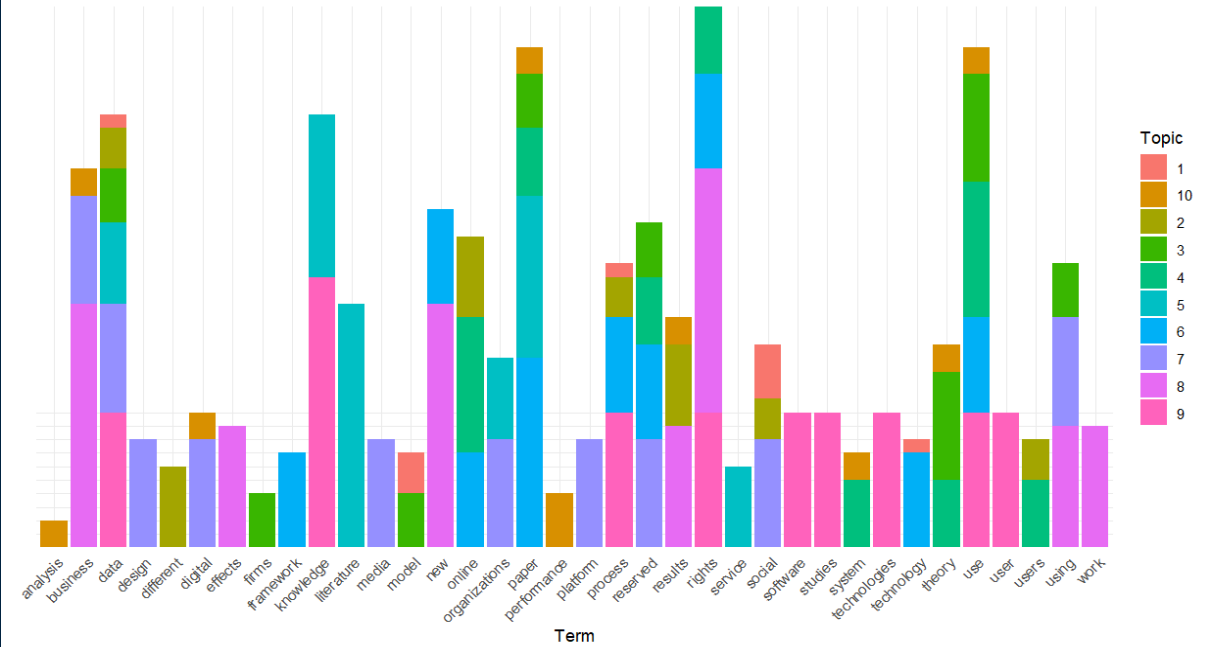
\includegraphics[width=5.20833in,height=\textheight]{images/freqTermsPerTopicSingleGraph.png}

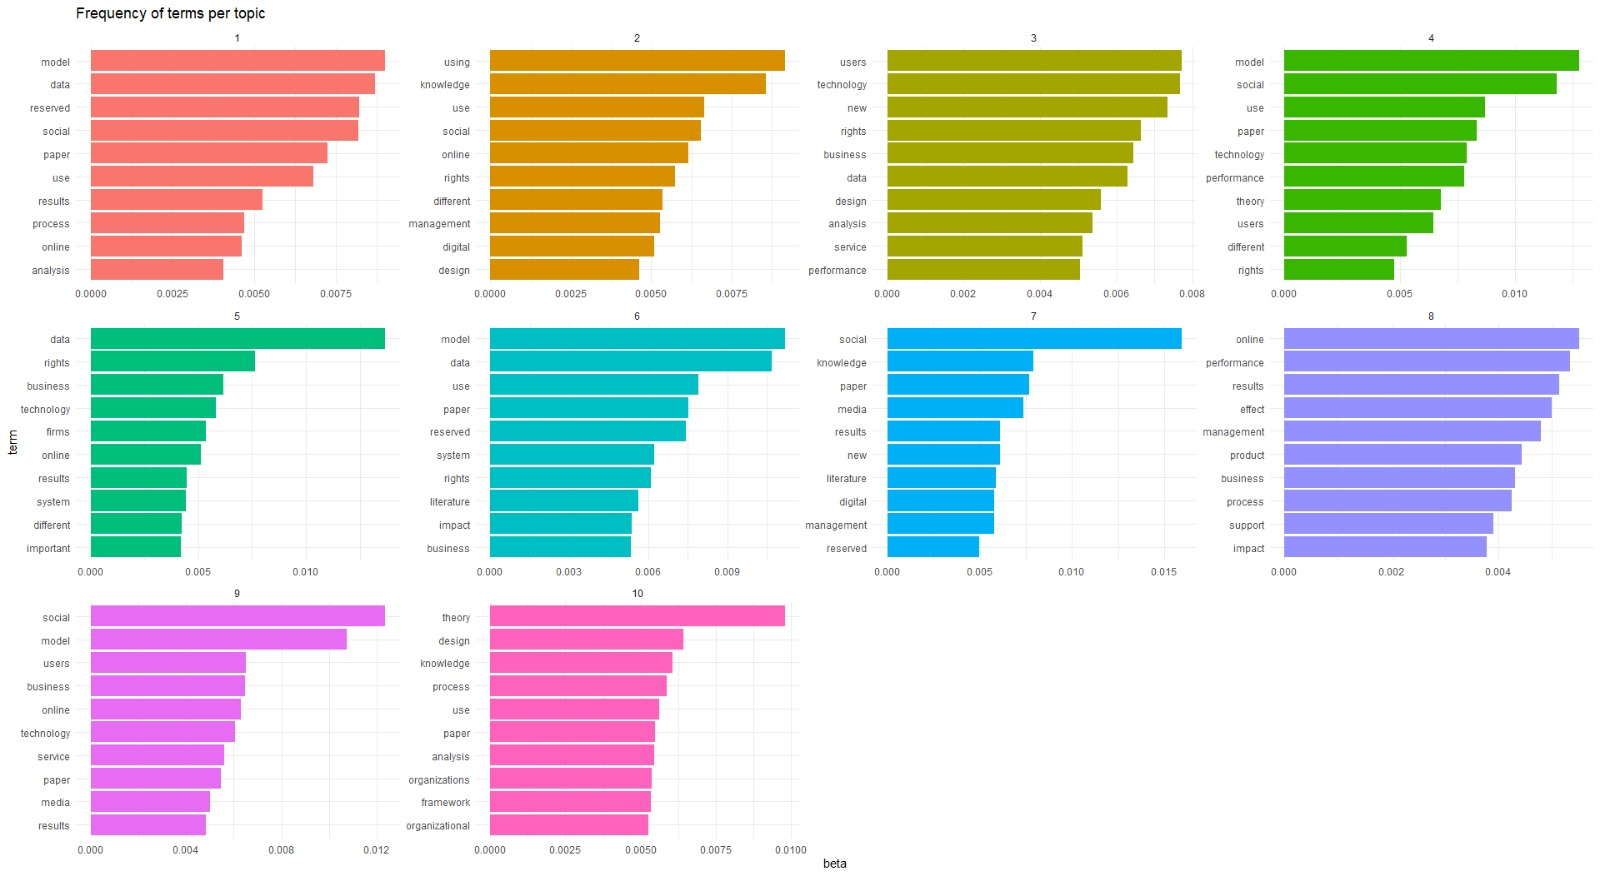
\includegraphics[width=5.20833in,height=\textheight]{images/freqTermsPerTopic-01.jpg}

Topics such as data analytics, social impact, knowledge management and
user behaviour are prominent, with terms such as ``online'', ``model''
and ``rights'' offering valuable insight into the ongoing debates and
areas being explored within the IS field.

\newpage{}

\hypertarget{evolution-of-is-research-topics-and-themes-2011-2020}{%
\subsection{2. Evolution of IS Research Topics and Themes
(2011-2020)}\label{evolution-of-is-research-topics-and-themes-2011-2020}}

Using Structural Topic Modelling (STM) we were able to track the
evolution of prevalent topics over the past decade.

An overview of these topics and their overall expected topic proportions
can be seen below.

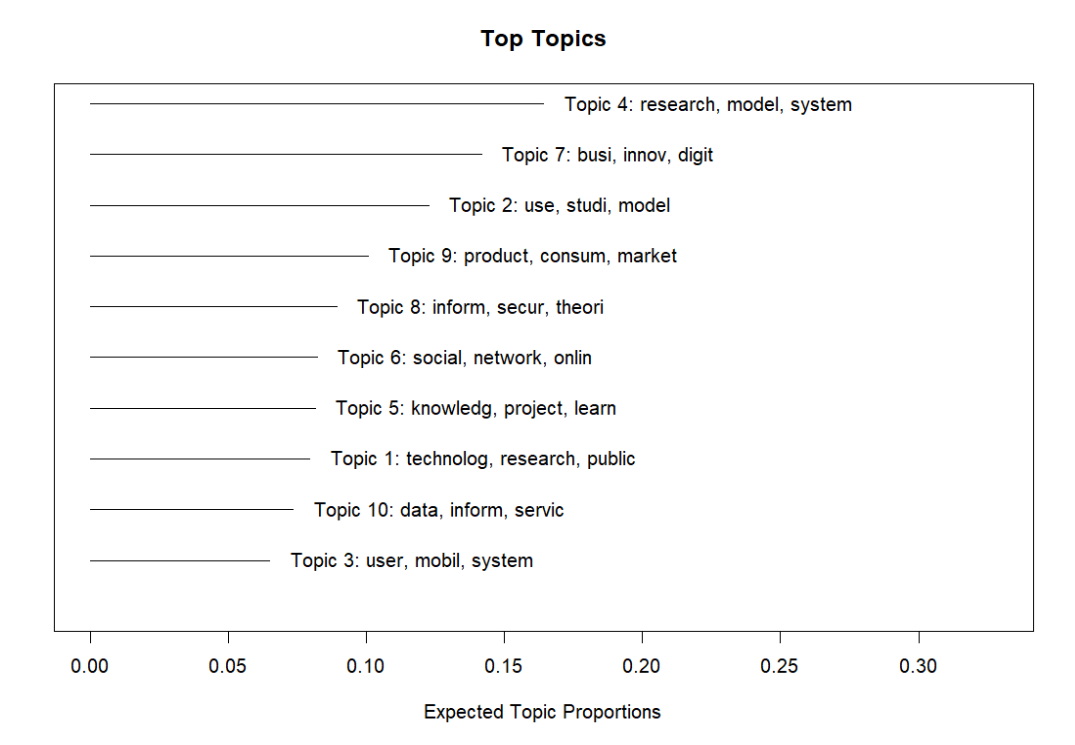
\includegraphics{images/STMTopicOverview.png}

\hypertarget{topic-1-technology-and-digitization}{%
\subsubsection{Topic 1: Technology and
Digitization}\label{topic-1-technology-and-digitization}}

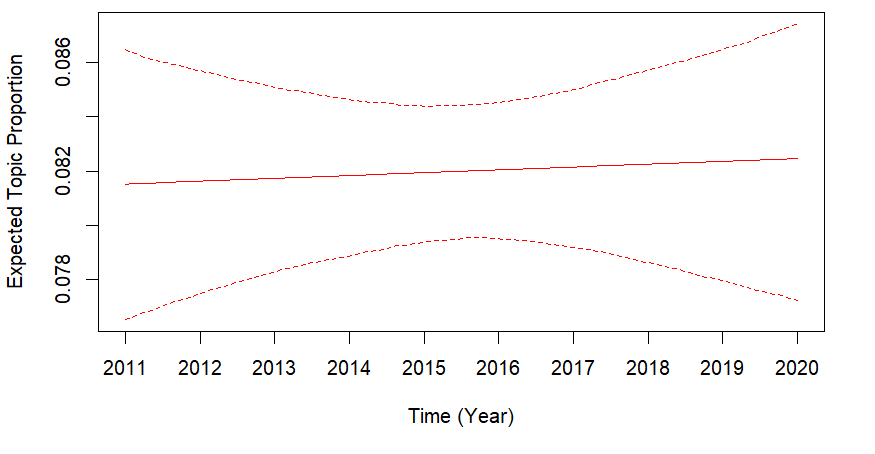
\includegraphics{images/topic1.png}

This topic entails discussions surrounding technology adoption, digital
transformation and ICT initiatives in a variety of sectors including
public services.

Keywords include technology, research, public, digit, develop and ICT
are prevalent in this topic. ~

This topic has had a slight increase in prevalence from 2011 to 2020.

\hypertarget{topic-2-user-influence-and-effects}{%
\subsubsection{Topic 2: User Influence and
Effects}\label{topic-2-user-influence-and-effects}}

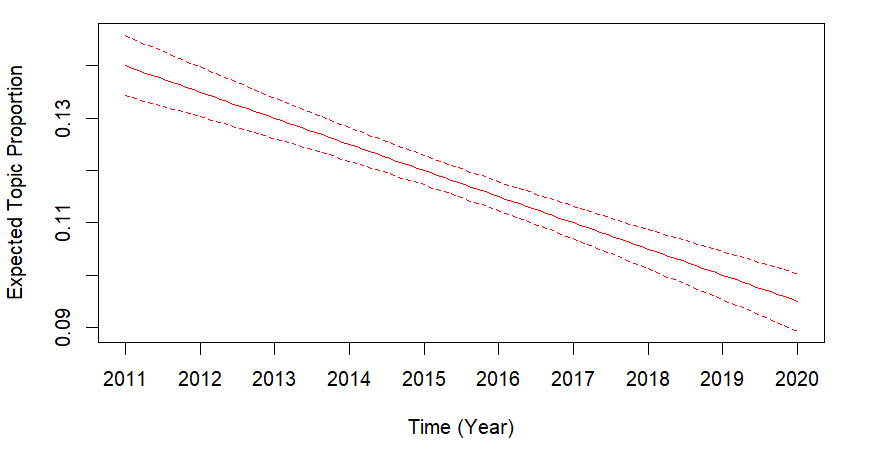
\includegraphics{images/topic2.png}

This topic focuses on understanding user behaviour, the factors
influencing technology adoption and the effect of technology use on
individuals and organisations.

Keywords include use, study, model, research, influence and factor.

This topic has had a steep decrease in prevalence from 2011 to 2020.

\hypertarget{topic-3-mobile-and-app-design}{%
\subsubsection{Topic 3: Mobile and App
Design}\label{topic-3-mobile-and-app-design}}

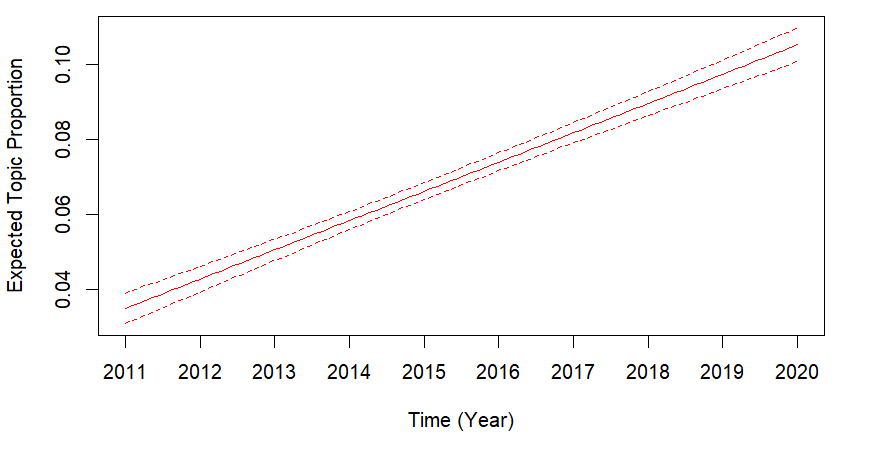
\includegraphics{images/topic3.png}

This topic explores mobile technology, app design, user experience and
the impact of mobile applications on user behavior and interaction.

Keywords include user, mobile, system, design, experience and app.

This topic has had a steep increase in prevalence from 2011 to 2020.

\hypertarget{topic-4-research-methodologies-and-approaches}{%
\subsubsection{Topic 4: Research Methodologies and
Approaches}\label{topic-4-research-methodologies-and-approaches}}

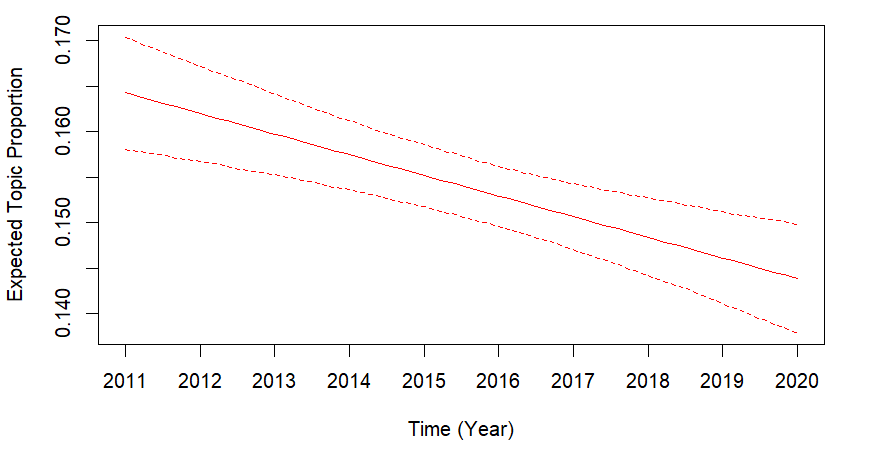
\includegraphics{images/topic4.png}

This topic revolves around research methodologies, system design
approaches and process modeling techniques used in IS research.

Keywords include research, model, system, design, approach and process.

This topic has had a steep decrease in prevalence from 2011 to 2020.

\hypertarget{topic-5-knowledge-management-and-collaboration}{%
\subsubsection{Topic 5: Knowledge Management and
Collaboration}\label{topic-5-knowledge-management-and-collaboration}}

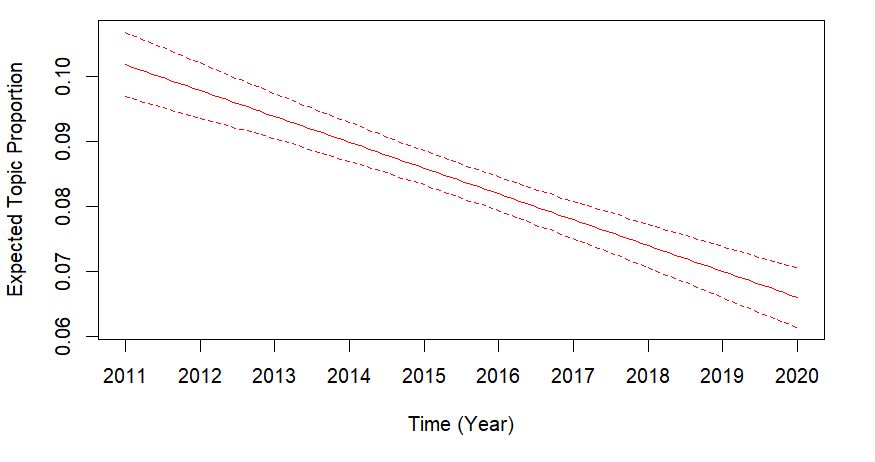
\includegraphics{images/topic5.png}

This topic emphasises knowledge management practices, collaborative
project development, software engineering and team dynamics in IS
projects.

Keywords include knowledge, project, learn, develop, software and team.

This topic has had a steep decrease in prevalence from 2011 to 2020.

\hypertarget{topic-6-social-media-and-online-communities}{%
\subsubsection{Topic 6: Social Media and Online
Communities}\label{topic-6-social-media-and-online-communities}}

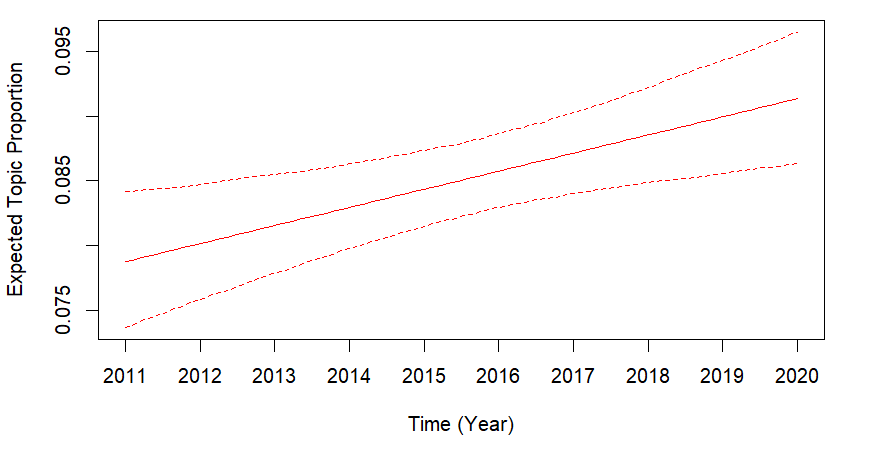
\includegraphics{images/topic6.png}

This topic focuses on social media platforms, online networks, user
interactions and the spread of information on said platforms.

Keywords include social, network, online, media, user and information.

This topic has had a steep increase in prevalence from 2011 to 2020.

\hypertarget{topic-7-business-innovation-and-digital-transformation}{%
\subsubsection{Topic 7: Business Innovation and Digital
Transformation}\label{topic-7-business-innovation-and-digital-transformation}}

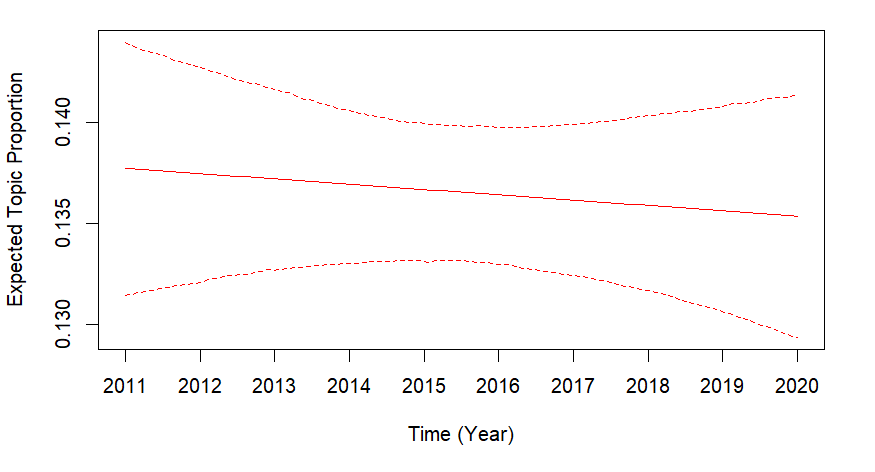
\includegraphics{images/topic7.png}

This topic explores business innovation, digital strategies and
organisational capabilities and value creation through digital
transformation initiatives.

Keywords include business, innovation, digital, firm, value and process.

This topic has had a gradual decrease in prevalence from 2011 to 2020.

\hypertarget{topic-8-information-security-and-risk-management}{%
\subsubsection{Topic 8: Information Security and Risk
Management}\label{topic-8-information-security-and-risk-management}}

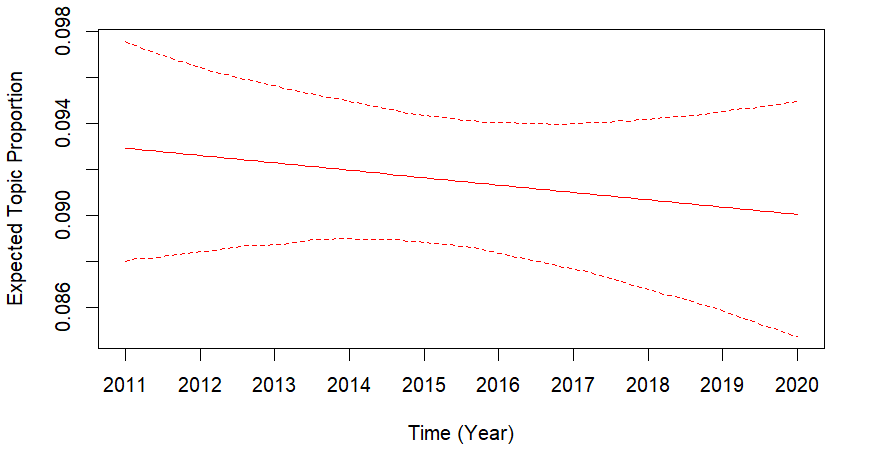
\includegraphics{images/topic8.png}

This topic addresses information security theories, practices, risk
management strategies and organisational responses to security threats
and challenges.

Keywords include information, security, practice, work and organisation.

This topic has had a gradual decrease in prevalence from 2011 to 2020.

\hypertarget{topic-9-e-commerce-and-consumer-behaviour}{%
\subsubsection{Topic 9: E-commerce and Consumer
Behaviour}\label{topic-9-e-commerce-and-consumer-behaviour}}

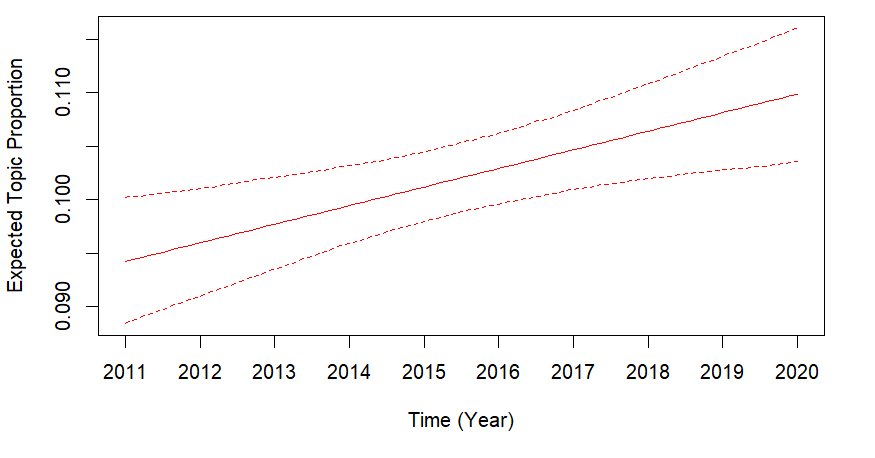
\includegraphics{images/topic9.png}

This topic examines e-commerce trends, consumer behaviour, market
dynamics, online product reviews and the effects of online shopping on
businesses and consumers.

Keywords include product, consumer, market, custom, online and effect.

This topic has had a steep increase in prevalence from 2011 to 2020.

\hypertarget{topic-10-data-management-and-healthcare}{%
\subsubsection{Topic 10: Data Management and
Healthcare}\label{topic-10-data-management-and-healthcare}}

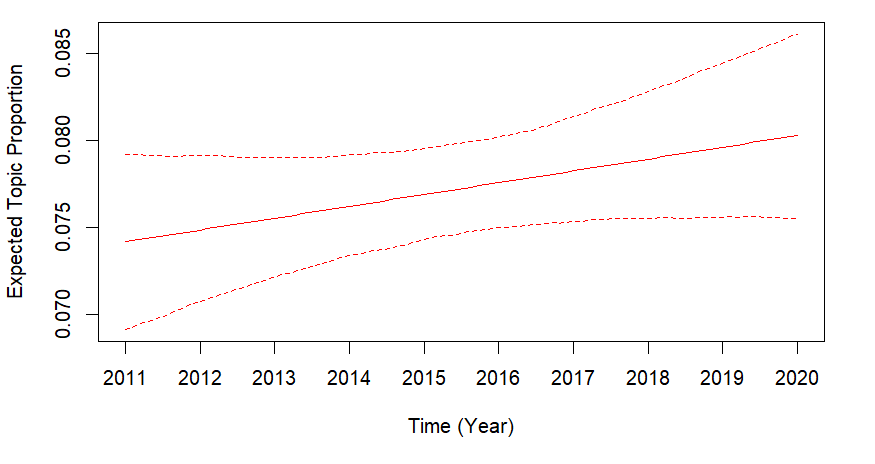
\includegraphics{images/topic10.png}

This topic covers data management practices, information services, risk
assessment and healthcare informatics.

Keywords include data, information, service, system, risk and health. ~

This topic has had a gradual increase in prevalence from 2011 to 2020.

\newpage{}

\hypertarget{most-productive-authors-and-journals-in-the-field-of-is}{%
\subsection{\texorpdfstring{\textbf{3. Most Productive Authors and
Journals in the Field of
IS}}{3. Most Productive Authors and Journals in the Field of IS}}\label{most-productive-authors-and-journals-in-the-field-of-is}}

Multiple metrics can be used to measure Author productivity. This
includes

\hypertarget{publications-per-author}{%
\subsubsection{Publications per Author}\label{publications-per-author}}

The following graph displays the total count of publications written per
author for the top authors (\textgreater50 publications). This indicates
how many articles were published by each respective author. There are a
total of 45,345 publications written by 16,693 authors. This allows for
an average of 10.32 total publications per author. Yuan Li has published
the most articles, having been involved in the publication of 91
articles.

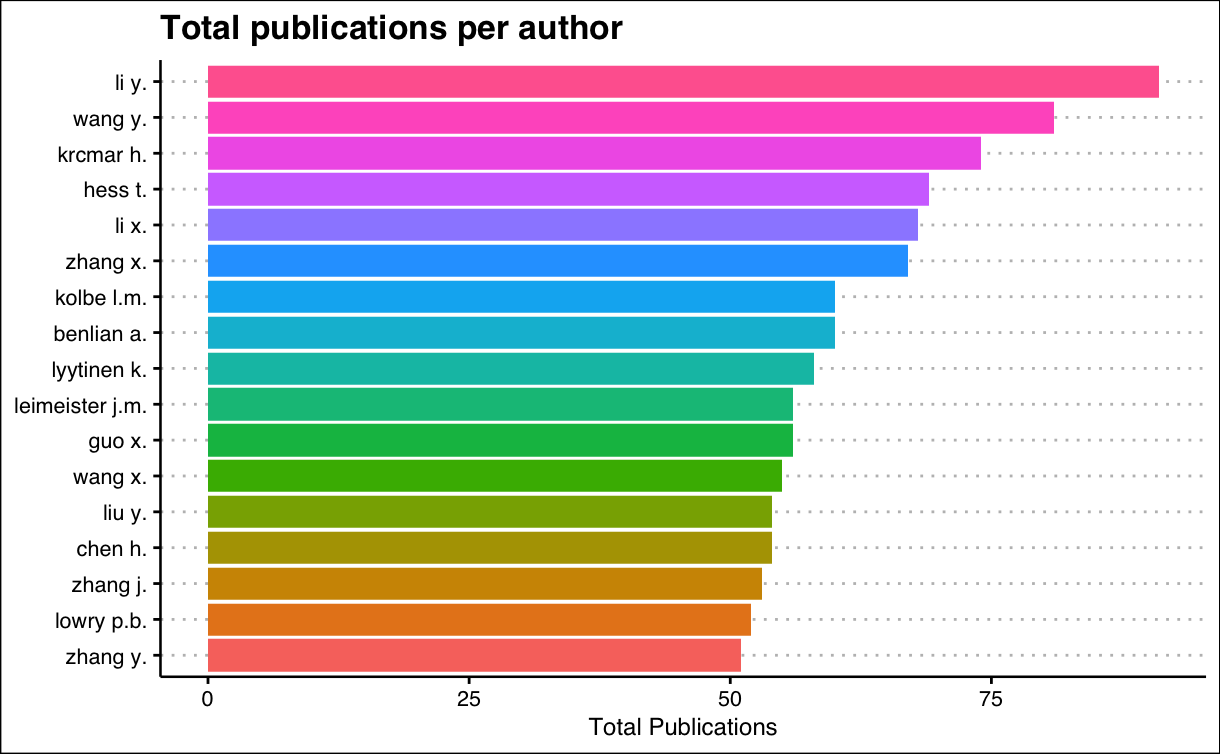
\includegraphics{images/pub_per_auth-01.png}

\hypertarget{publication-rate-per-author}{%
\subsubsection{Publication Rate per
Author}\label{publication-rate-per-author}}

The publication rate for each author was calculated by determining for
how long they were active (last publication - first publication),
followed by dividing their total publications. This shows us how
productive each author is/was throughout their academic career. The
average publication rate was 1.513, with the highest being Yuan Li at
\textasciitilde10 publications per year.

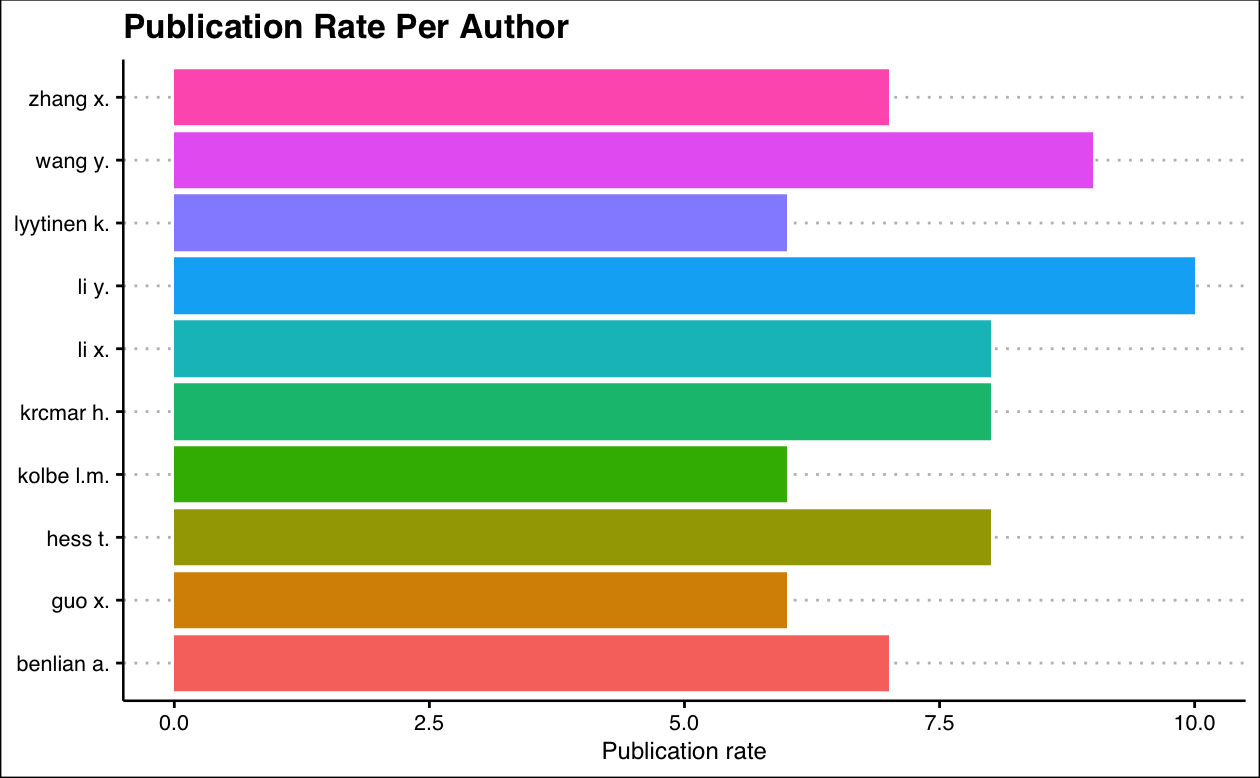
\includegraphics{images/pub_rate-01.png}

\hypertarget{citations-per-author}{%
\subsubsection{Citations Per author}\label{citations-per-author}}

The visualisation shows us which authors have been cited the most. With
Venkatesh, V., Morris, M. G., and Davis, G. B. having the most
citations. With the average author being cited \textasciitilde{} 21
times.

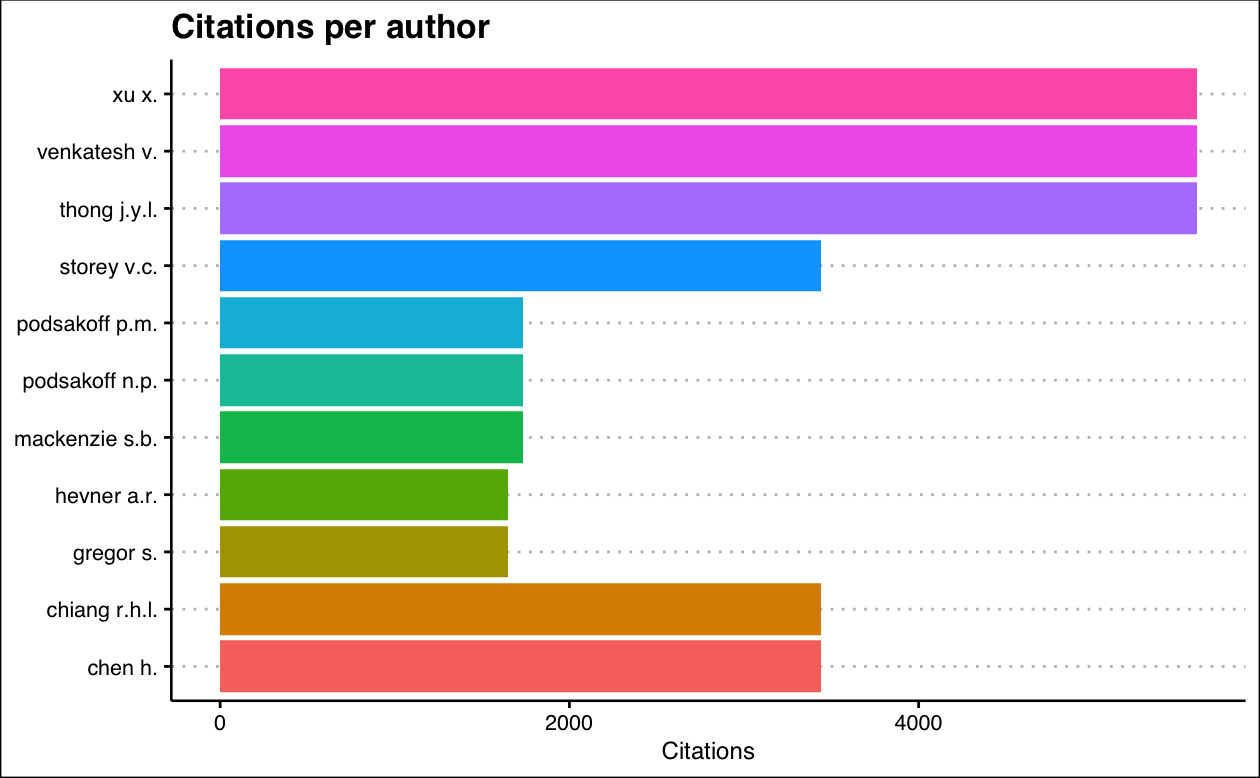
\includegraphics{images/cite_per_auth-01.png}

\hypertarget{publications-by-author-for-respective-journals}{%
\subsubsection{Publications by author for respective
Journals}\label{publications-by-author-for-respective-journals}}

As seen in the graph below, The MIS Quarterly has garnered the most
citations (74,687) despite only having the second highest publications
(555). The Information Systems Research was published the most articles
(567) but only received the second most citations (32,130). On average
the various journals had a mean publications of 365, and the average
total citations was 25,342. There is a strong positive correlation
between total publications and total citations, with a positive
correlation value of 0.772.

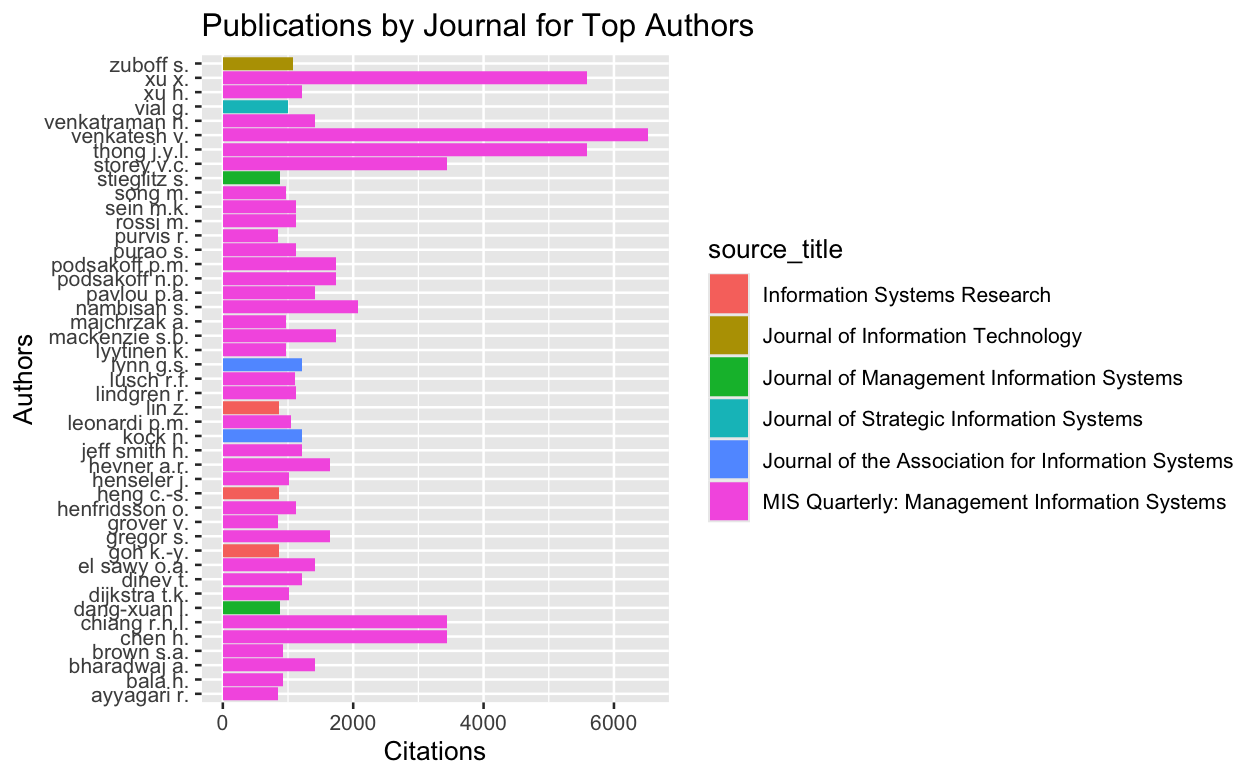
\includegraphics{images/pub_journ_auth.png}

\hypertarget{excluding-mis-quarterly}{%
\subsubsection{Excluding MIS Quarterly}\label{excluding-mis-quarterly}}

When excluding the MIS Quarterly from the visualisation, it provides
valuable insight into the number of publications, authors and citations
for the remaining journals. This allows us to compare these journals
without skewing the graph with data from the MIS Quarterly. Furthermore,
this shows us the top authors for these journals respectively.

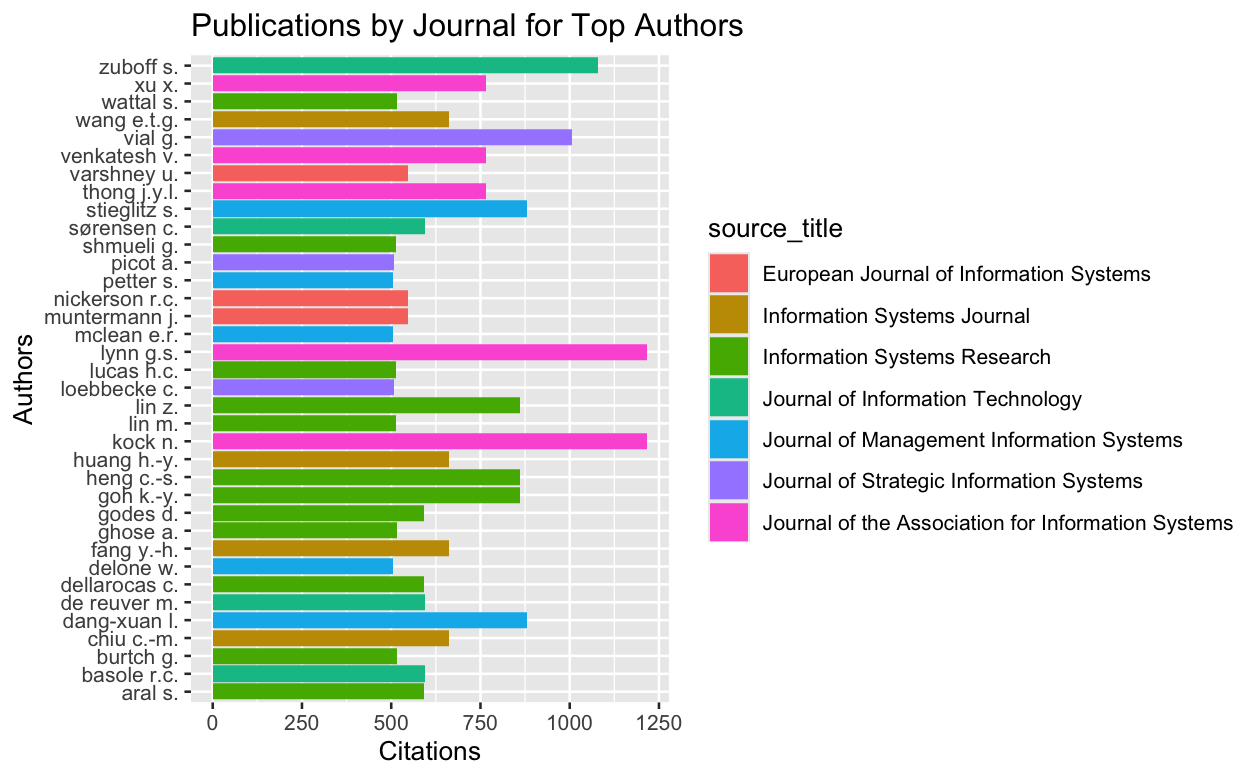
\includegraphics{images/pub_journ_ex.png}

\hypertarget{total-publications-and-citations-per-journal}{%
\subsubsection{Total Publications and Citations per
Journal}\label{total-publications-and-citations-per-journal}}

This graph displays the Total Publications per journal as well as the
total citations. Again, showcasing that MIS Quarterly has been cited the
most, and the Information Systems Research having the most publications.

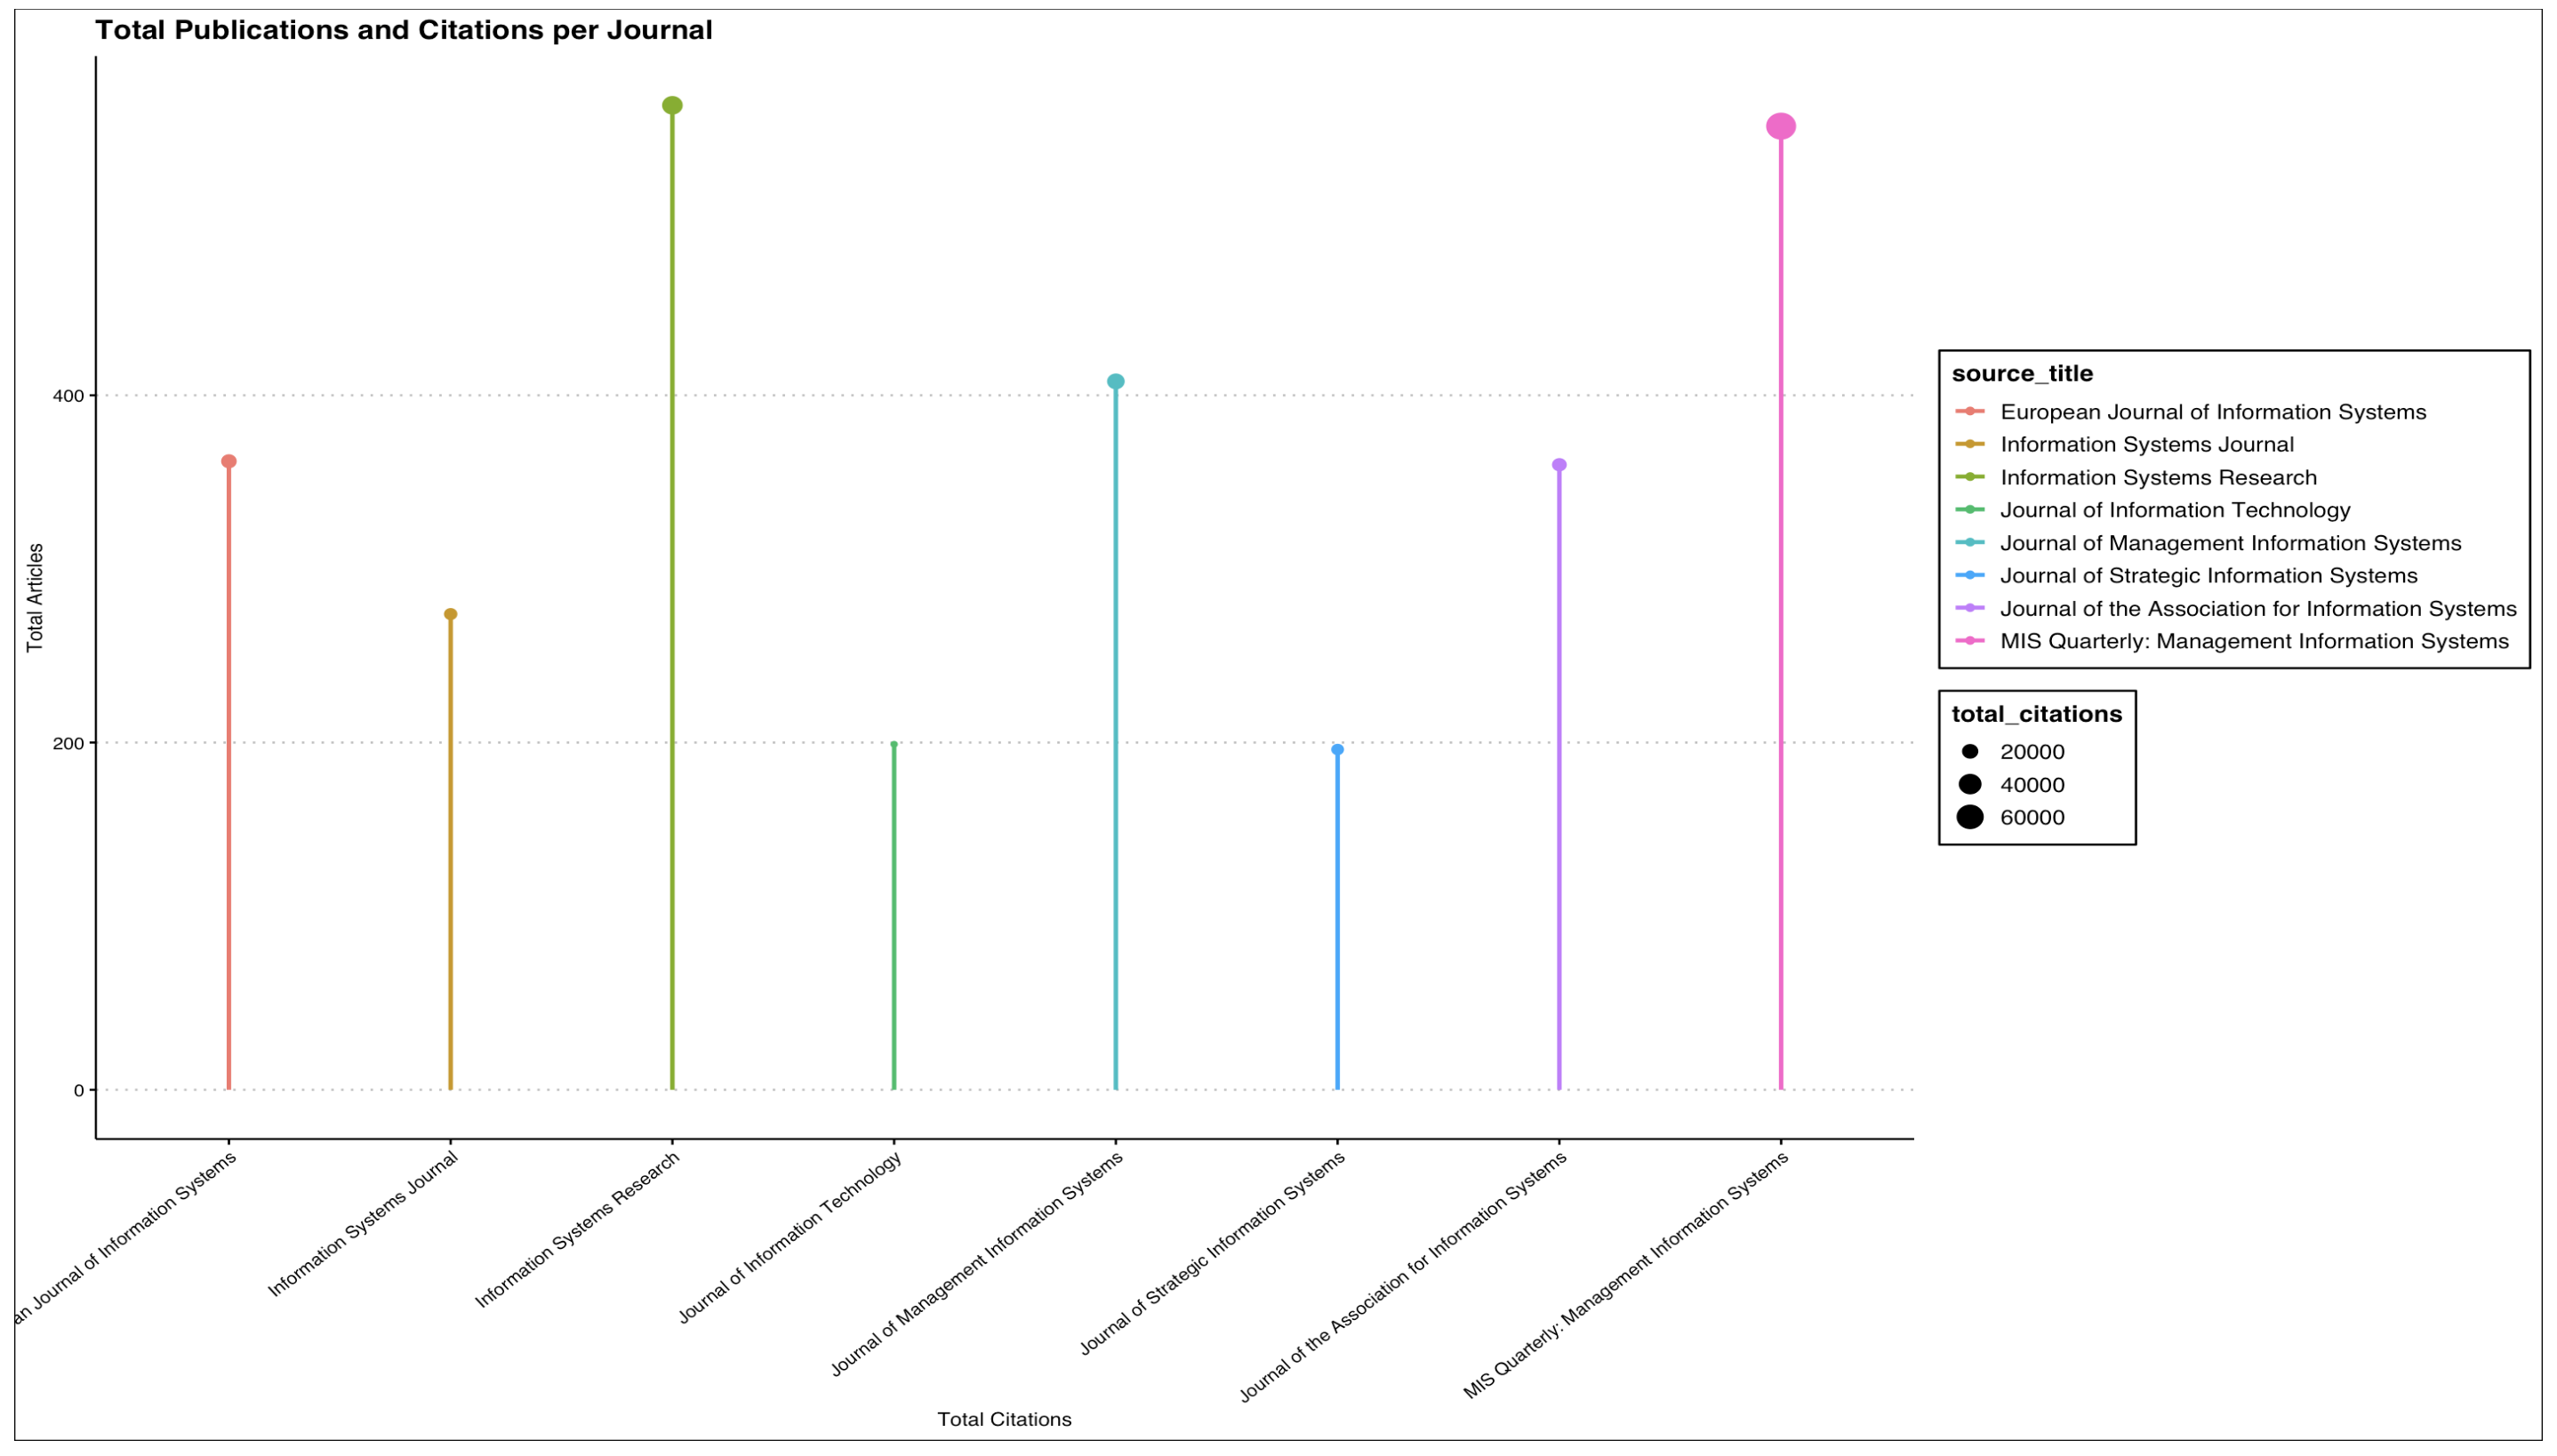
\includegraphics{images/pub_cite_journ.png}

\hypertarget{most-frequent-sources}{%
\subsubsection{Most frequent sources}\label{most-frequent-sources}}

The following graph plots the top 15 most sources in the data. These are
the journals and conferences that have the most number of papers
published under there name. The graph shows that the yearly Americas
Conference of Information Systems seems to produce the most papers.

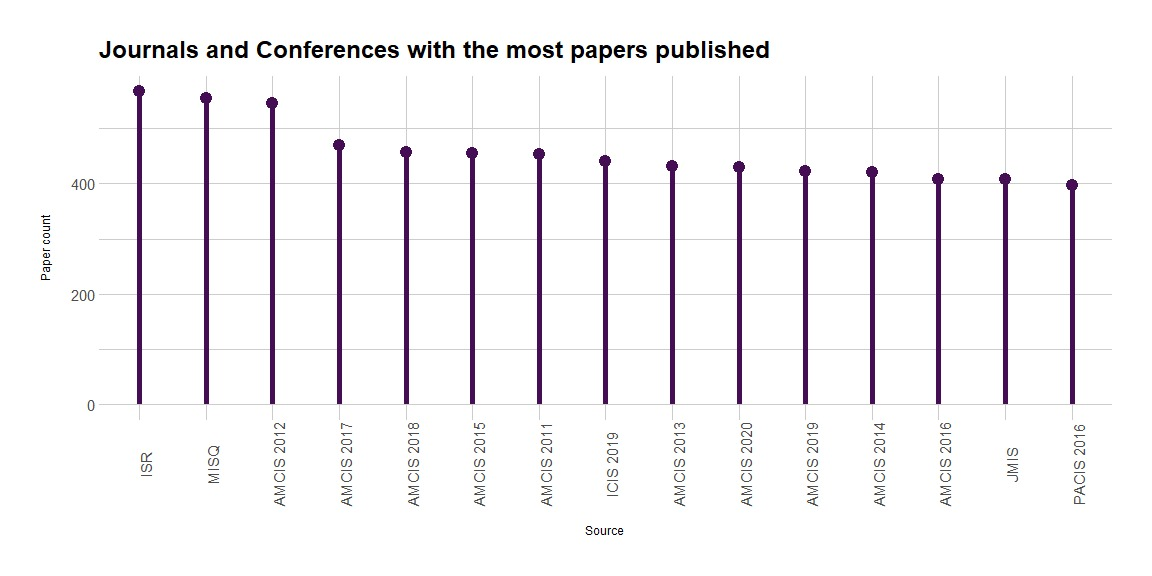
\includegraphics[width=5.72917in,height=\textheight]{images/JournalsandConfrMostPapersPublished.jpg}

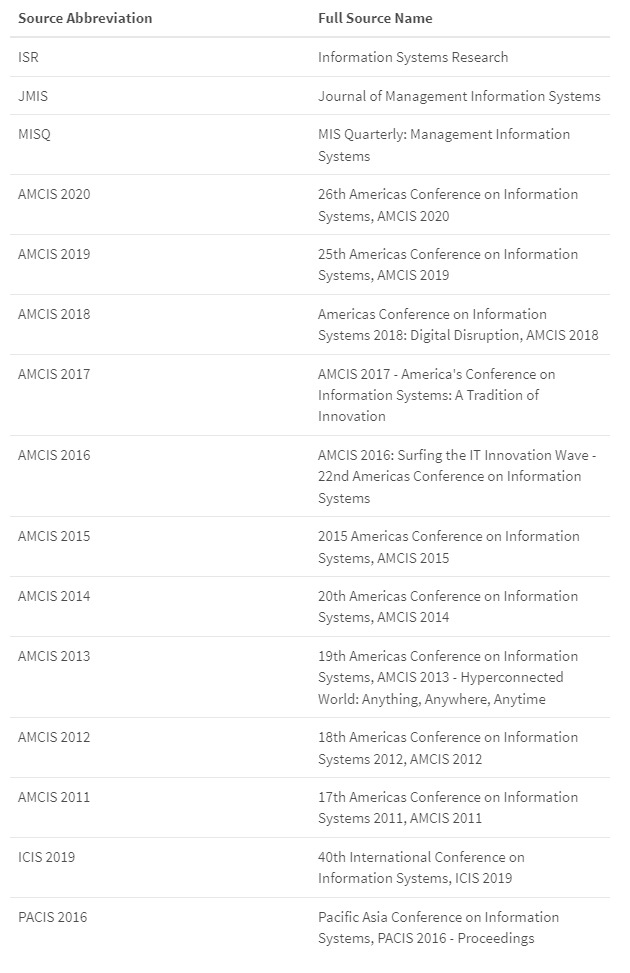
\includegraphics[width=3.125in,height=\textheight]{images/freqSourceAbrv.jpg}

\hypertarget{most-influential-sources}{%
\subsubsection{Most influential
sources}\label{most-influential-sources}}

The graph below shows the sources that produce the most cited papers.
The total citations per article in the source was tallied to calculate
the influence per source.

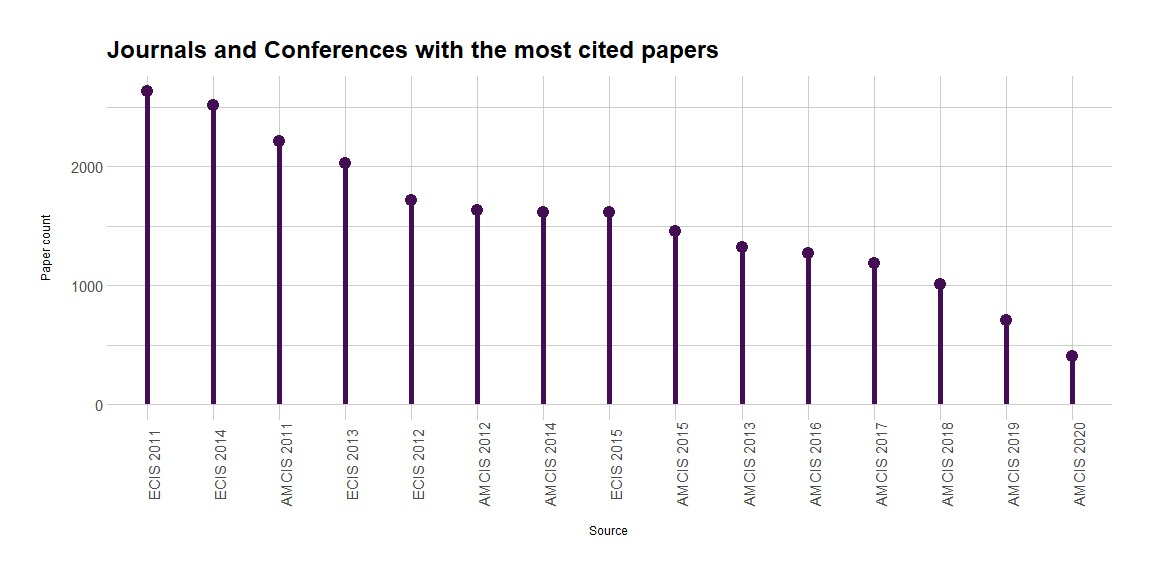
\includegraphics[width=5.72917in,height=\textheight]{images/InfJournalsandConfrMostPapersPublished.jpg}

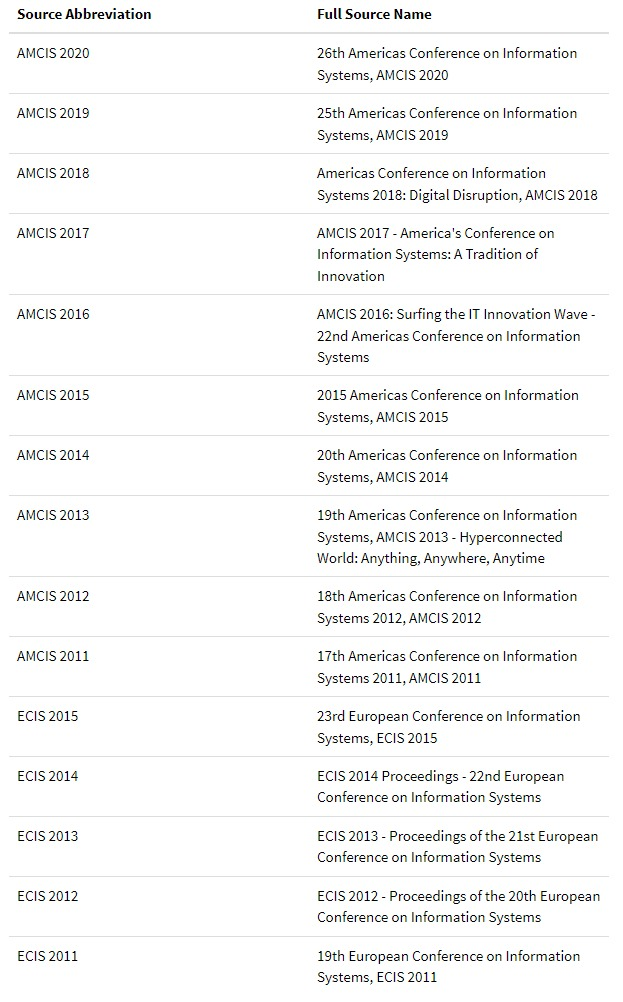
\includegraphics[width=3.125in,height=\textheight]{images/infSourceAbrv.jpg}

\newpage{}

\hypertarget{impact-of-is-research-measured-by-citation-counts}{%
\subsection{4. Impact of IS research (Measured by Citation
Counts)}\label{impact-of-is-research-measured-by-citation-counts}}

\hypertarget{top-cited-overall}{%
\subsubsection{Top cited overall}\label{top-cited-overall}}

The table below shows the top 10 most cited papers over the ten years.
The top most cited paper has 5 593 citations, and was published in 2012,
showing it has had a clear impact since its release. The paper explores
the theory of acceptance and use of information technology, which is
often used to explore new developments within the information systems
field. The other papers in the top 10 invlove a mixture of exploring the
practical implications of technology as well as contributing to
theoretical research.

\begin{figure}

{\centering 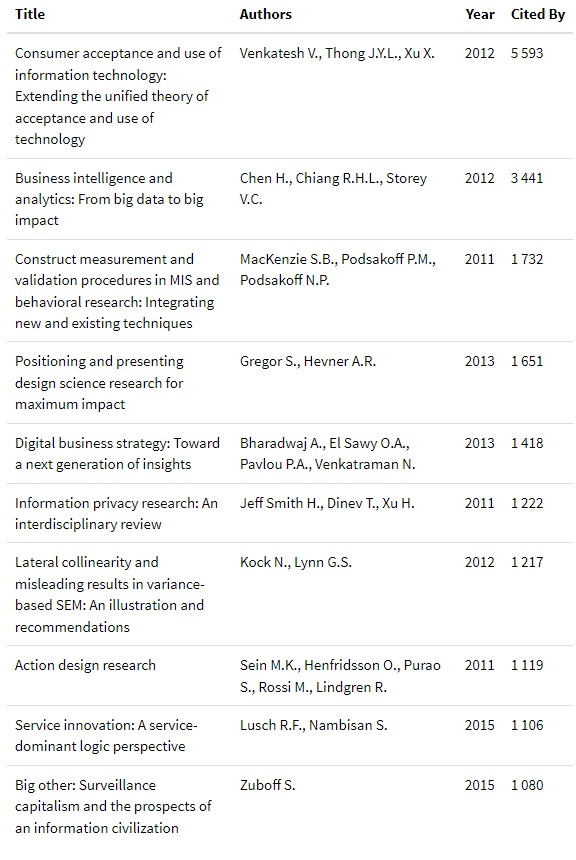
\includegraphics[width=4.6875in,height=\textheight]{images/topCitedOverall.jpg}

}

\end{figure}

\hypertarget{top-cited-papers-for-each-year}{%
\subsubsection{Top cited papers for each
year}\label{top-cited-papers-for-each-year}}

The table below displays the paper from each year with the most
citations. This table shows that generally older papers tend to have
more citations than newer ones, but this can be attributed to them being
around for longer. Their is an overall trend of research about how
technology and people interact, with a focus on digitisation in more
recent years.

\begin{figure}

{\centering 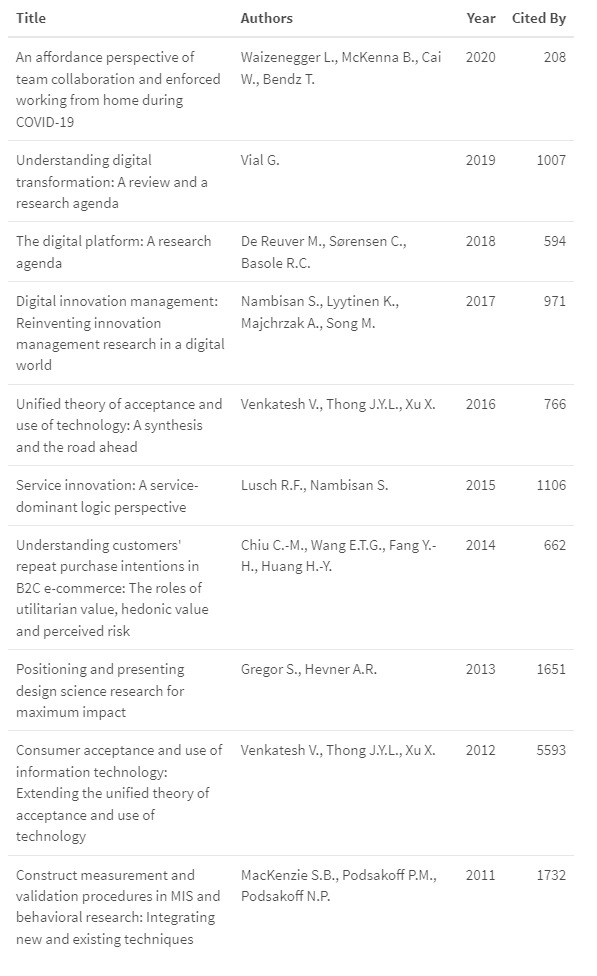
\includegraphics[width=4.6875in,height=\textheight]{images/topCitedPerYear.jpg}

}

\end{figure}

\newpage{}

\hypertarget{most-frequent-keywords-in-is-and-how-they-have-changed-over-time}{%
\subsection{\texorpdfstring{5. \textbf{Most Frequent Keywords in IS and
How They Have Changed Over
Time}}{5. Most Frequent Keywords in IS and How They Have Changed Over Time}}\label{most-frequent-keywords-in-is-and-how-they-have-changed-over-time}}

There are two type of keywords that will be analysed from the data
source: author keywords and index keywords. Author keywords are the
terms that the author chooses to represent their paper. Index keywords
are terms that terms that are chosen by indexers to categorise the paper
witin the database and aid in database organisation. In this section, we
will compare the two types amongst them and against each other.

\hypertarget{author-keywords}{%
\subsubsection{Author Keywords}\label{author-keywords}}

\hypertarget{over-10-years}{%
\subsubsection{Over 10 years}\label{over-10-years}}

\begin{figure}

{\centering 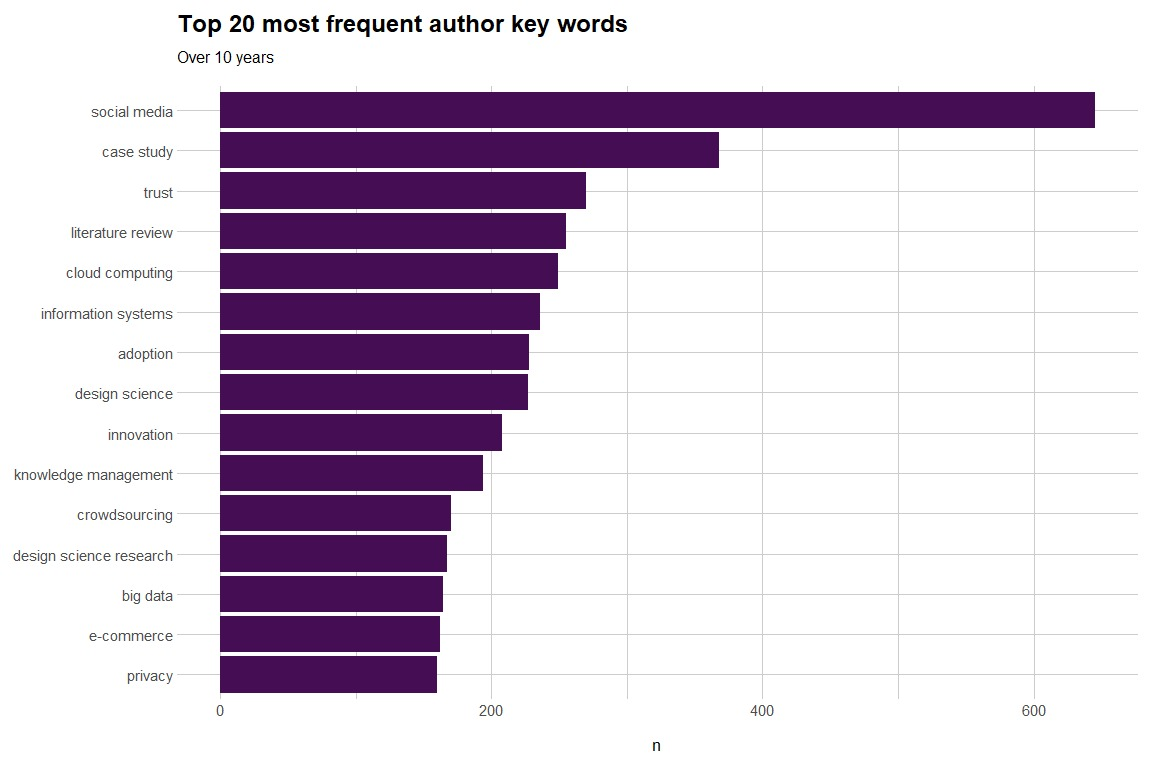
\includegraphics[width=4.16667in,height=\textheight]{images/top20mostfreqauthorkeywords.jpg}

}

\end{figure}

\begin{figure}

{\centering 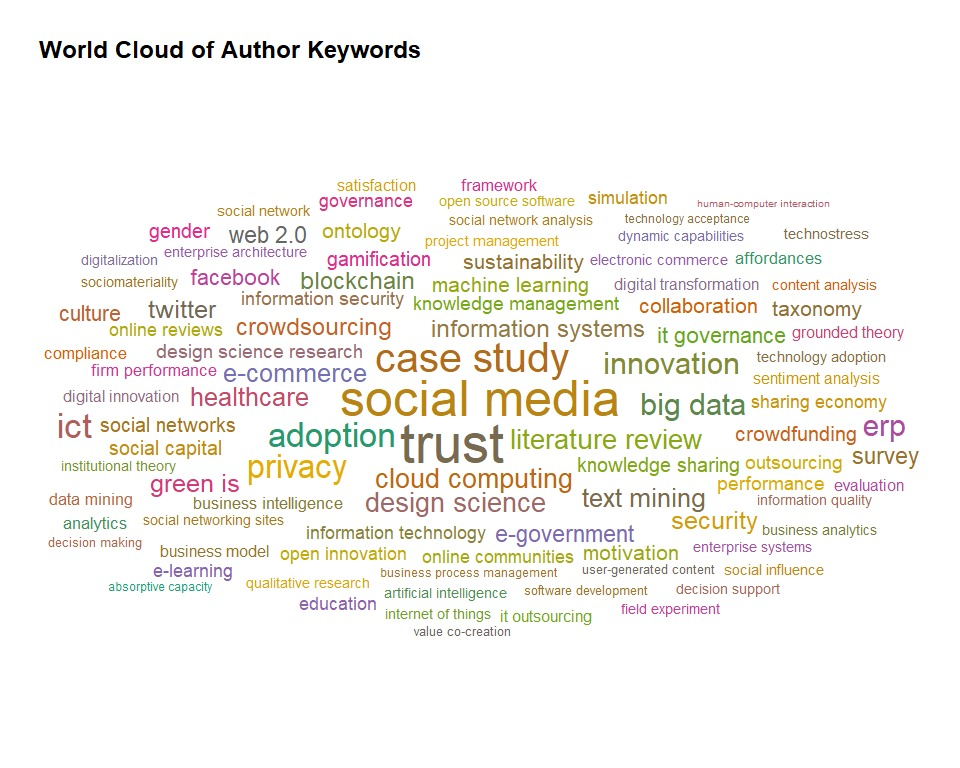
\includegraphics[width=4.16667in,height=\textheight]{images/top20mostfreqauthorkeywordsWordCloud-01.jpg}

}

\end{figure}

The above graph and word cloud shows the most frequent author keywords
in IS ver 10 years. The clear leader is social media and this can be
attributed to the increased in interest in social media itself and
social media analysis throughout the 2010s.The word cloud visualises the
keywords in a way that is easier to see which were most prevalent over
the years, as well as showing some of the other keywords studied, but
not as frequently.

\hypertarget{by-year}{%
\subsubsection{By year}\label{by-year}}

\begin{figure}

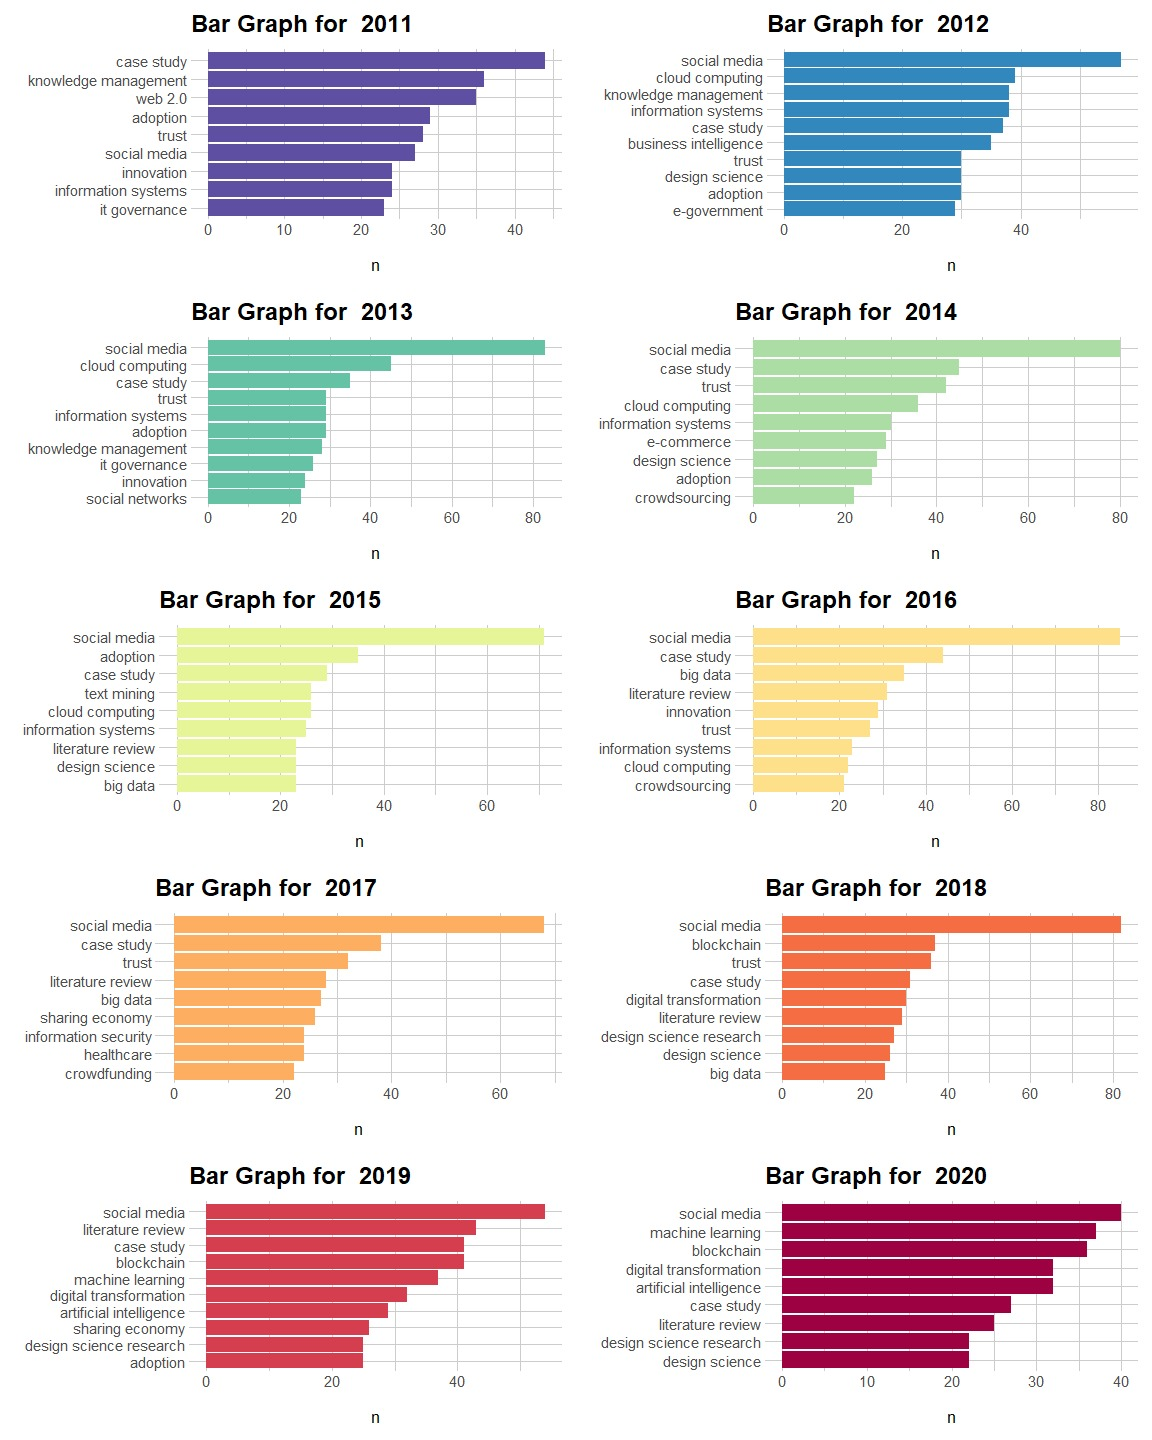
\includegraphics[width=5.72917in,height=\textheight]{images/bargraphbyyearAuthor-01.jpg} \hfill{}

\end{figure}

The above graphs show the top author keywords for each year. Social
media has stayed the most popular across all years, except for 2011,
contributing the fact that it is also the most frequent keyword over
all. Each year the keywords shift to include more topics that were
prevalent in that year, from knowledge management and cloud computing in
2011 and 2012, to machine learning, blockchain and artificial
intelligence in 2019 and 2020. This shows the IS field is constantly
evolving in the research that is done and the topics that are covered.

\hypertarget{open-access-vs-limited-access}{%
\subsubsection{Open Access vs Limited
Access}\label{open-access-vs-limited-access}}

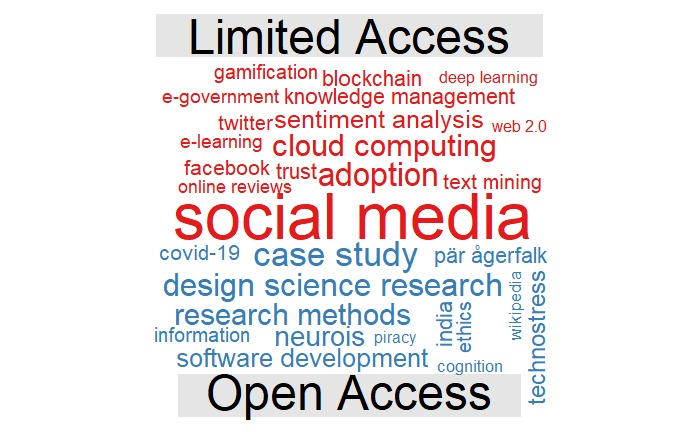
\includegraphics[width=5.20833in,height=\textheight]{images/authorsLimitedvsOpen-01.jpg}

The above word cloud compared the keywords that are most found in open
access papers versus papers with limited access. The graph shows that
many of the case studies and research methods are found in open access
papers, whereas the specific trends, such as cloud computing, blockchain
and social media are more often found in limited access papers.

\hypertarget{conference-papers-vs-journal-papers}{%
\subsubsection{Conference Papers vs Journal
Papers}\label{conference-papers-vs-journal-papers}}

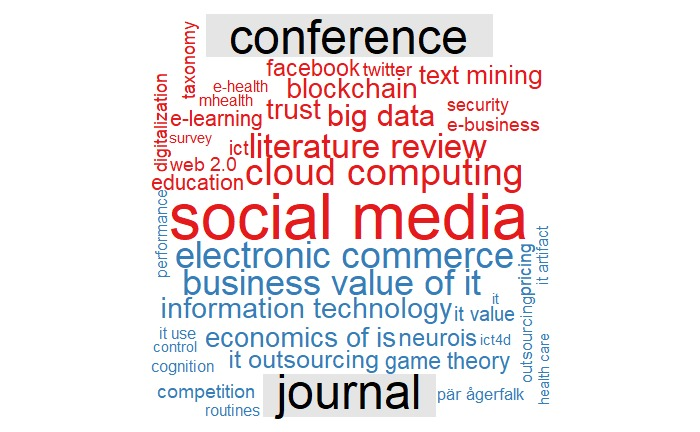
\includegraphics[width=5.20833in,height=\textheight]{images/authorsConferencevsJournal-01.jpg}

The above word cloud compared the keywords that are most found in papers
publicized in a journal versus papers published at a conference. The
graph shows that many of the papers related to theory and business and
economics related problems are published in journals, whereas the more
general topics of scoial media and big data are found more often in
conference papers.

\hypertarget{index-key-phrases}{%
\subsubsection{Index Key Phrases}\label{index-key-phrases}}

This section explores the index keywords in the same way author keywords
were explored.

\hypertarget{over-10-years-1}{%
\subsubsection{Over 10 years}\label{over-10-years-1}}

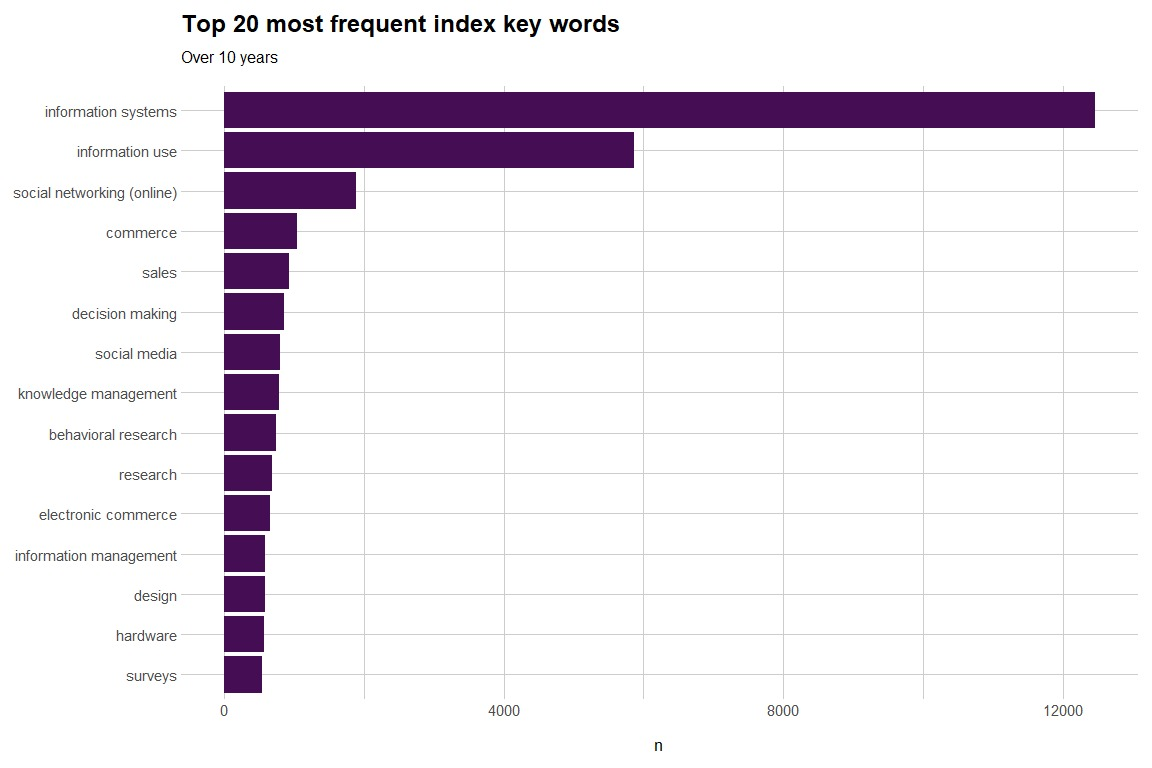
\includegraphics[width=5.20833in,height=\textheight]{images/Indextop20mostfreqkeywords.jpg}

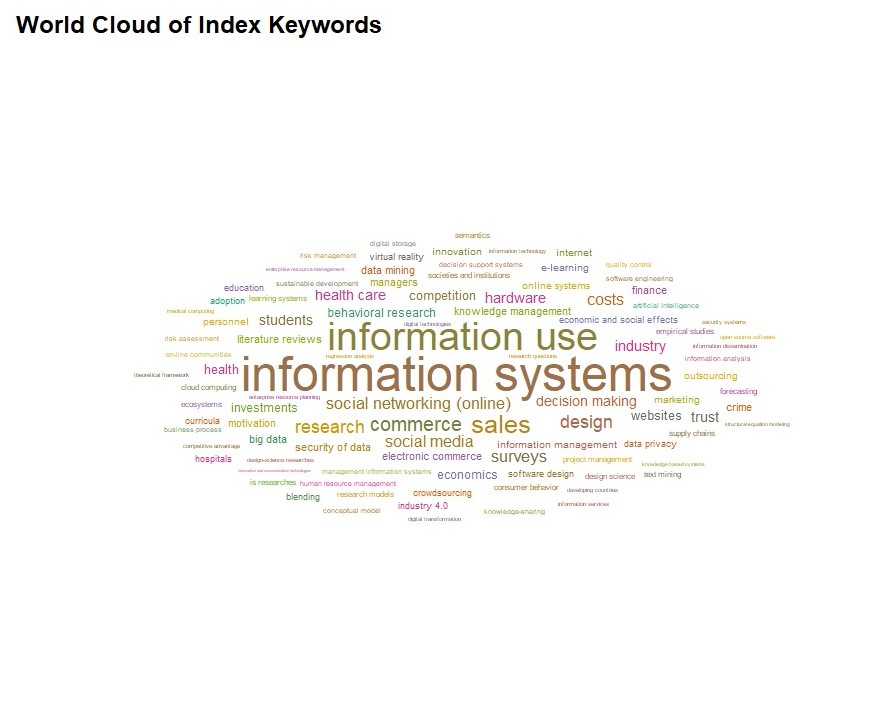
\includegraphics[width=5.20833in,height=\textheight]{images/Indextop20mostfreqkeywordsWordCloud.jpg}

The above graph and word cloud shows the most frequent index keywords in
IS over 10 years. The clear leader is information systems and this is
because these key words are used more for paper classification, and all
of them fall into the category of information systems. Social media and
social networking still feature quite highly in these keywords. The
index keyword word cloud shows that there is a broader variety in index
keywords, but there is a clear most frequent few and many only briefly
mentioned.

\hypertarget{by-year-1}{%
\subsubsection{By Year}\label{by-year-1}}

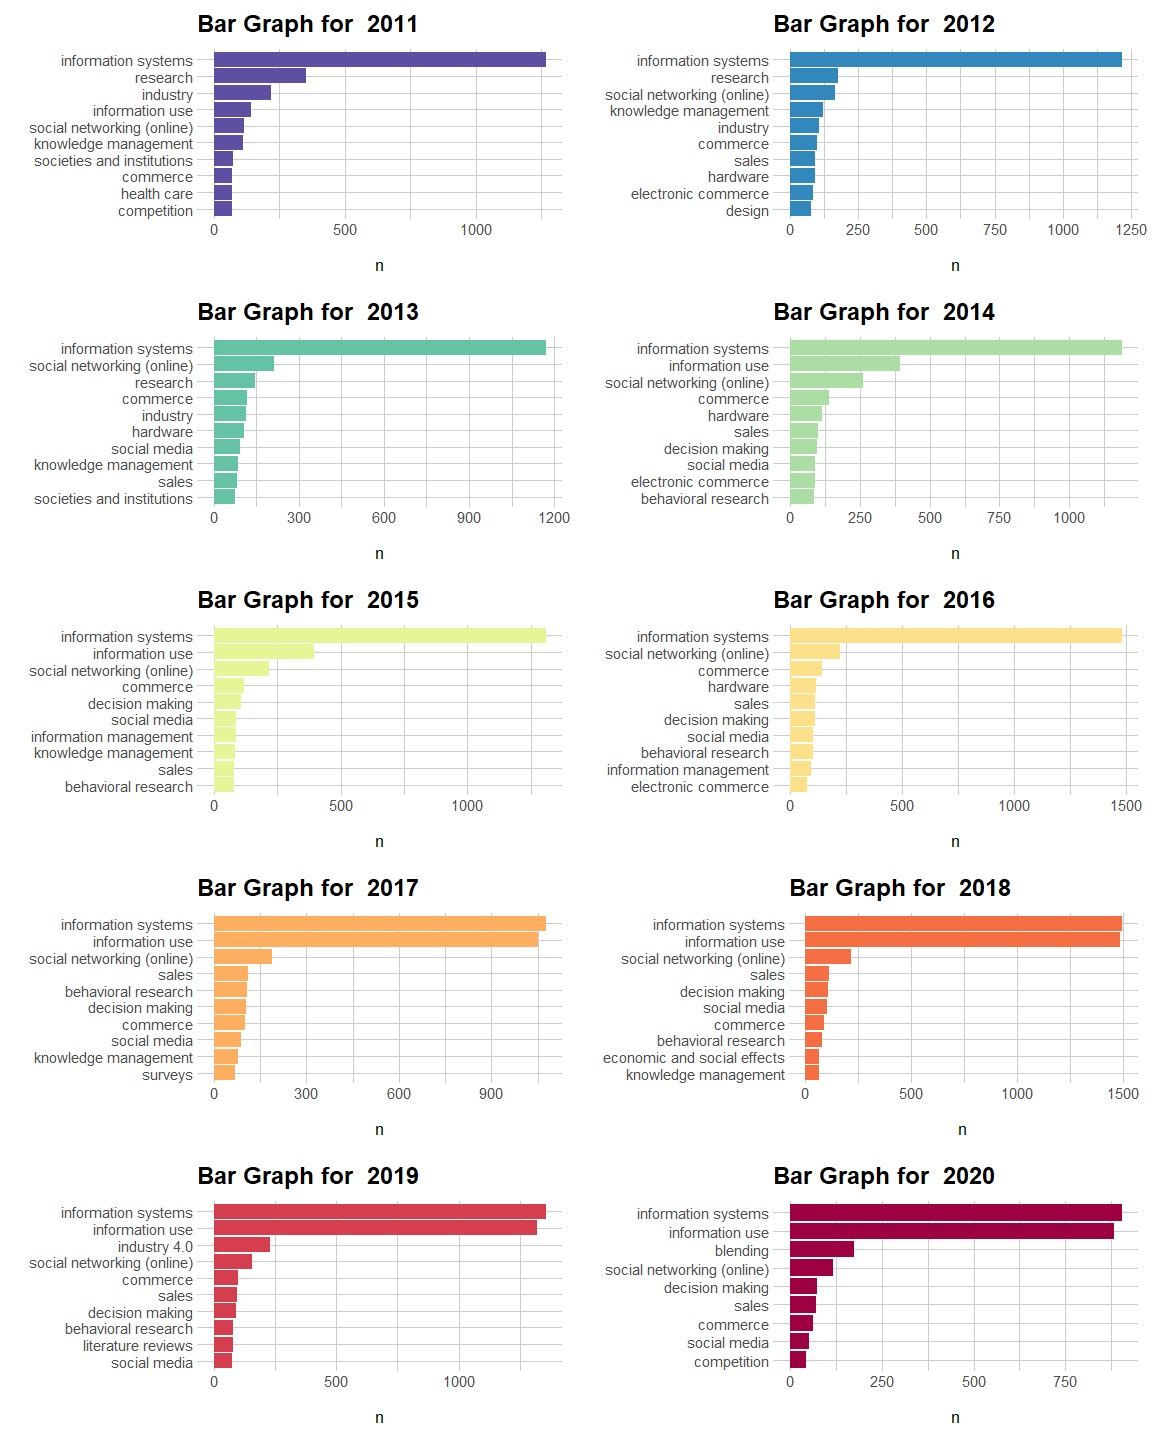
\includegraphics[width=5.20833in,height=\textheight]{images/bargraphbyyearIndex.jpg}

The above graphs show the top index keywords for each year. Information
systems has stayed the most popular across all years, because of the
reason discussed above. Each year the second most popular key word often
shifts between information use and social networking. This graph also
highlights the difference in the yearly author keywords and index
keywords, as these graphs have more generic keywords that the author
keywords.

\hypertarget{open-access-vs-limited-access-1}{%
\subsubsection{Open Access vs Limited
Access}\label{open-access-vs-limited-access-1}}

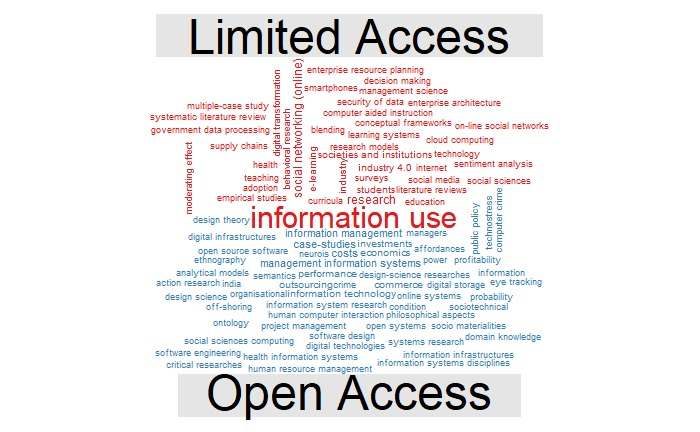
\includegraphics[width=5.20833in,height=\textheight]{images/indexLimitedvsOpen.jpg}

The above word cloud compared the keywords that are most found in open
access papers versus papers with limited access. The figure shows that
there is not as clear a difference between the index keywords for each
type, versus the author keywords for each type. There is not as much
variation in size in each type of paper. Open access seems to feature
more business related research, shown through keywords such as
management information systems, cost investments, and economics. Limited
access papers once again seem to focus on trends, such as social
networking and e-learning.

\hypertarget{conference-papers-vs-journal-papers-1}{%
\subsubsection{Conference Papers vs Journal
Papers}\label{conference-papers-vs-journal-papers-1}}

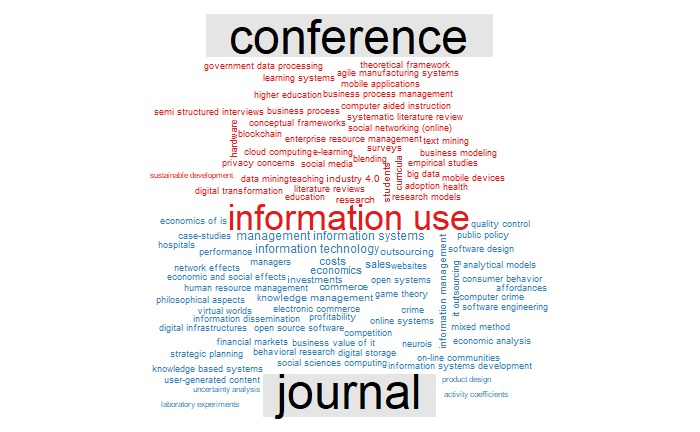
\includegraphics[width=5.20833in,height=\textheight]{images/indexConferencevsJournal.jpg}

The above word cloud compared the keywords that are most found in papers
publicized in a journal versus papers published at a conference. The
figure shows a similar trend as the open access vs limited access word
cloud, in that there is not as clear a difference in the keywords that
are featured in each type of paper.

\newpage{}

\hypertarget{relationship-between-specific-topics-and-themes-and-citation-counts}{%
\subsection{\texorpdfstring{6. \textbf{Relationship Between Specific
Topics and Themes and Citation
Counts}}{6. Relationship Between Specific Topics and Themes and Citation Counts}}\label{relationship-between-specific-topics-and-themes-and-citation-counts}}

\hypertarget{author-keywords-citations-counts}{%
\subsubsection{Author Keywords Citations
Counts}\label{author-keywords-citations-counts}}

The graph below displays the author keywords from articles which have
received more than 1500 citations. Here we can see 3 key words which
appears and has been cited dramatically more than others. Mobile
Internet as a key word was the most prevalent (\textasciitilde6,000),
highlighting its increased relevance in modern society. The Unified
theory of acceptance and use of technology (5,400) along with price
value (5,300) were also outliers.

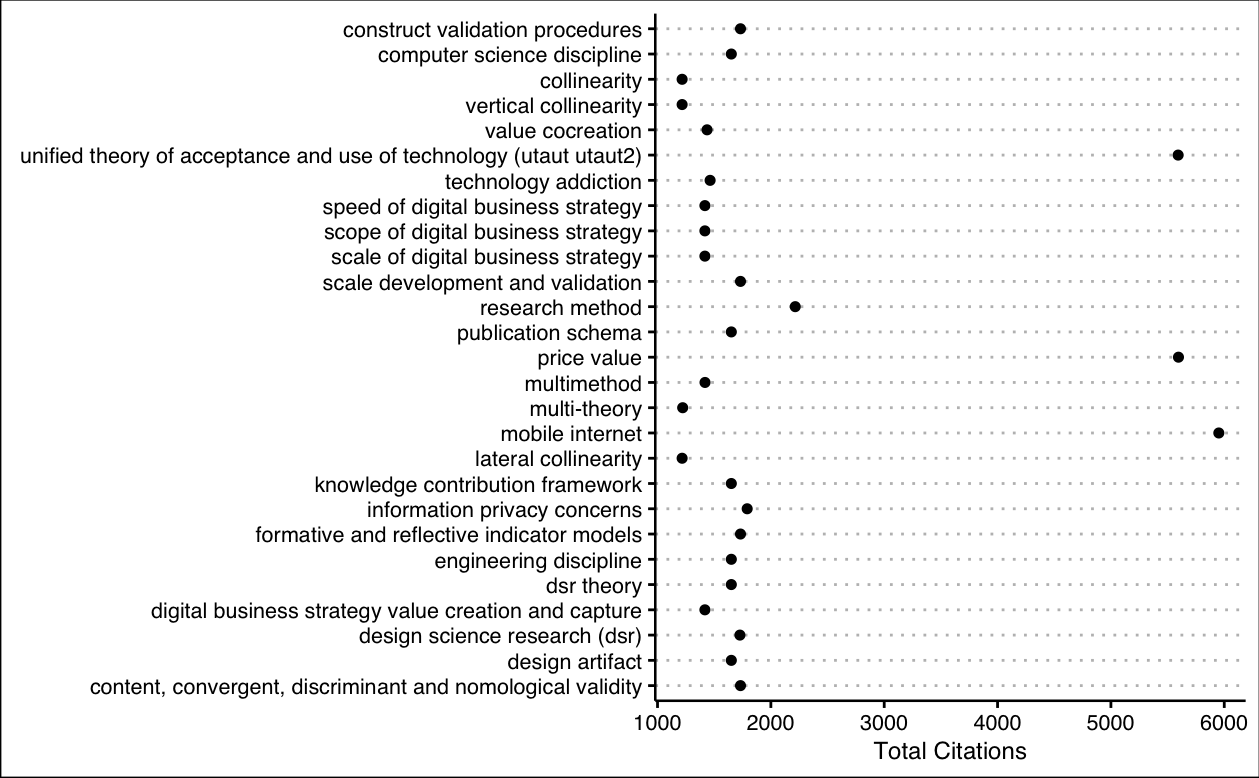
\includegraphics{images/auth_keys_scat.png}

\hypertarget{section}{%
\paragraph{}\label{section}}

\newpage{}

\hypertarget{relationship-between-authorship-patterns-and-research-impact-in-is-research}{%
\subsection{\texorpdfstring{7. \textbf{Relationship Between Authorship
Patterns and Research Impact in IS
Research}}{7. Relationship Between Authorship Patterns and Research Impact in IS Research}}\label{relationship-between-authorship-patterns-and-research-impact-in-is-research}}

\hypertarget{citations-per-author-count}{%
\subsubsection{Citations per Author
count}\label{citations-per-author-count}}

The following visualisation displays the amount of authors involved in a
publication, along with how many times the publications were cited. This
shows that multi-authorship publications tend to be cited more commonly,
with publications with 3 authors being cited the most. However, this
correlation between authorship and citation does not necessarily result
in direct causation. With results being heavily skewed by publications
such as the Unified Theory of Acceptance, written by Venkatesh, V.,
Morris, M. G., and Davis, G. B.

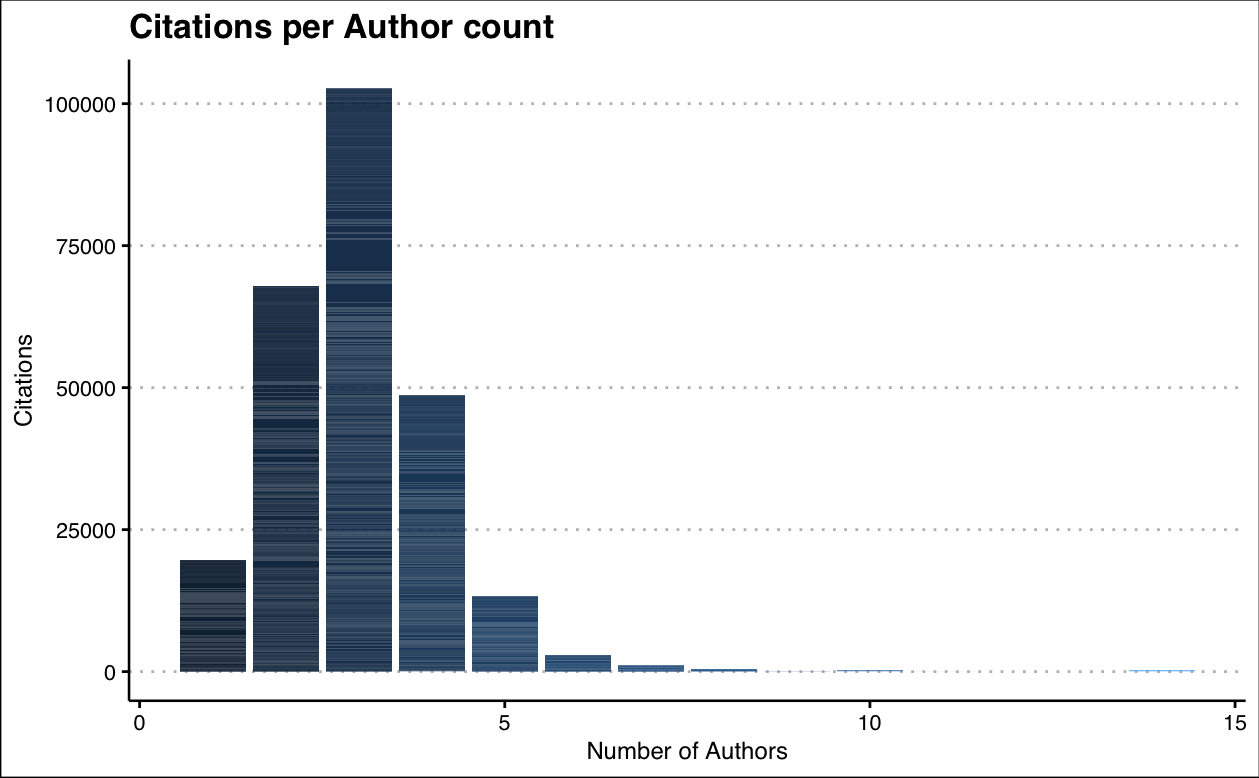
\includegraphics{images/cite_per_authship.png}

\hypertarget{citations-per-publishing-type}{%
\subsubsection{Citations per Publishing
type}\label{citations-per-publishing-type}}

The following graph displays the citations of publications from both
journals and conferences. It shows that publications in journals tend to
be more commonly cited when compared to conference publications.

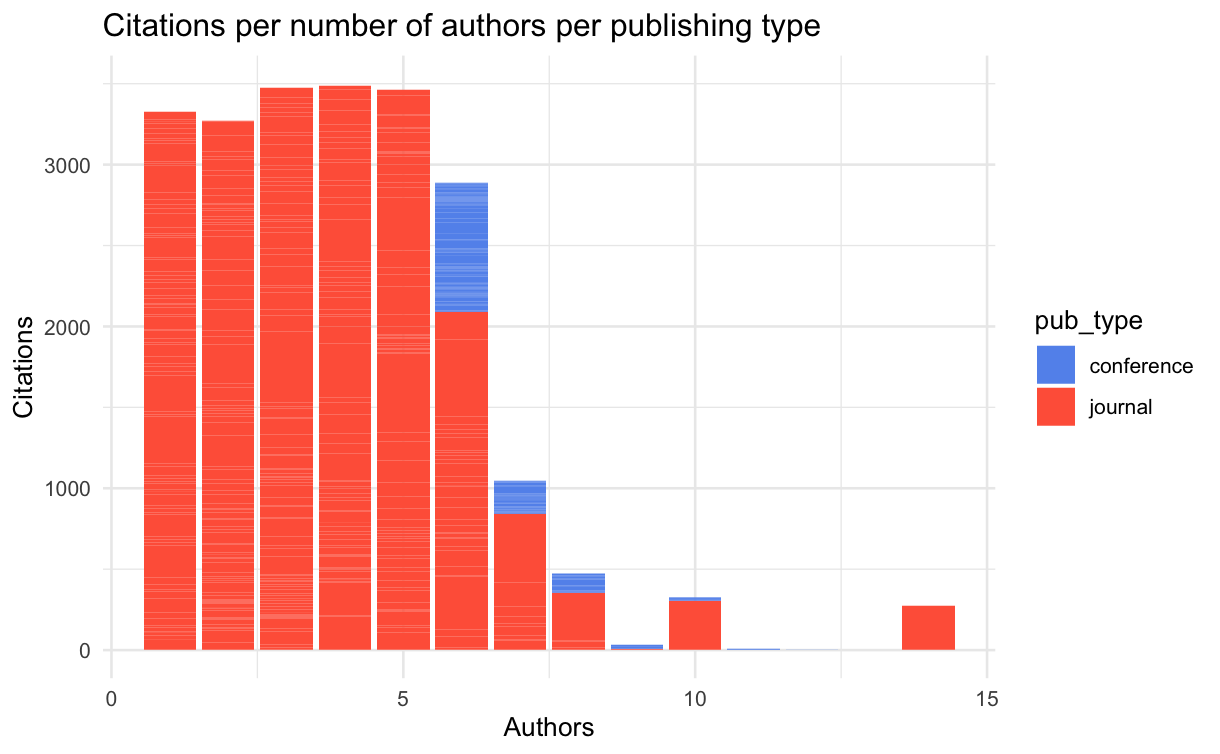
\includegraphics{images/cite_auth_type.png}

\newpage{}

\hypertarget{tonality-of-is-abstracts-by-topic}{%
\subsection{\texorpdfstring{8. \textbf{Tonality of IS Abstracts by
Topic}}{8. Tonality of IS Abstracts by Topic}}\label{tonality-of-is-abstracts-by-topic}}

Sentiment refers to the emotional tone behind some kind of text.
Sentiment analysis is the process of identifying the tone of text to
identify a dominant attitude. The following graphs are related to
investigating the sentiment for each topic identified through LDA.

\hypertarget{abstract-and-sentiments}{%
\subsubsection{Abstract and sentiments}\label{abstract-and-sentiments}}

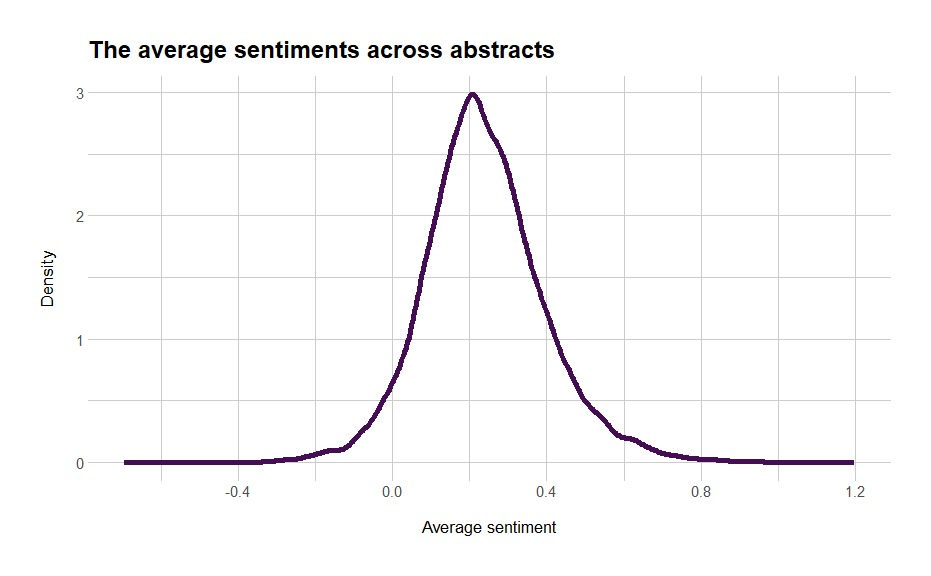
\includegraphics[width=4.6875in,height=\textheight]{images/aveSentiment.jpg}

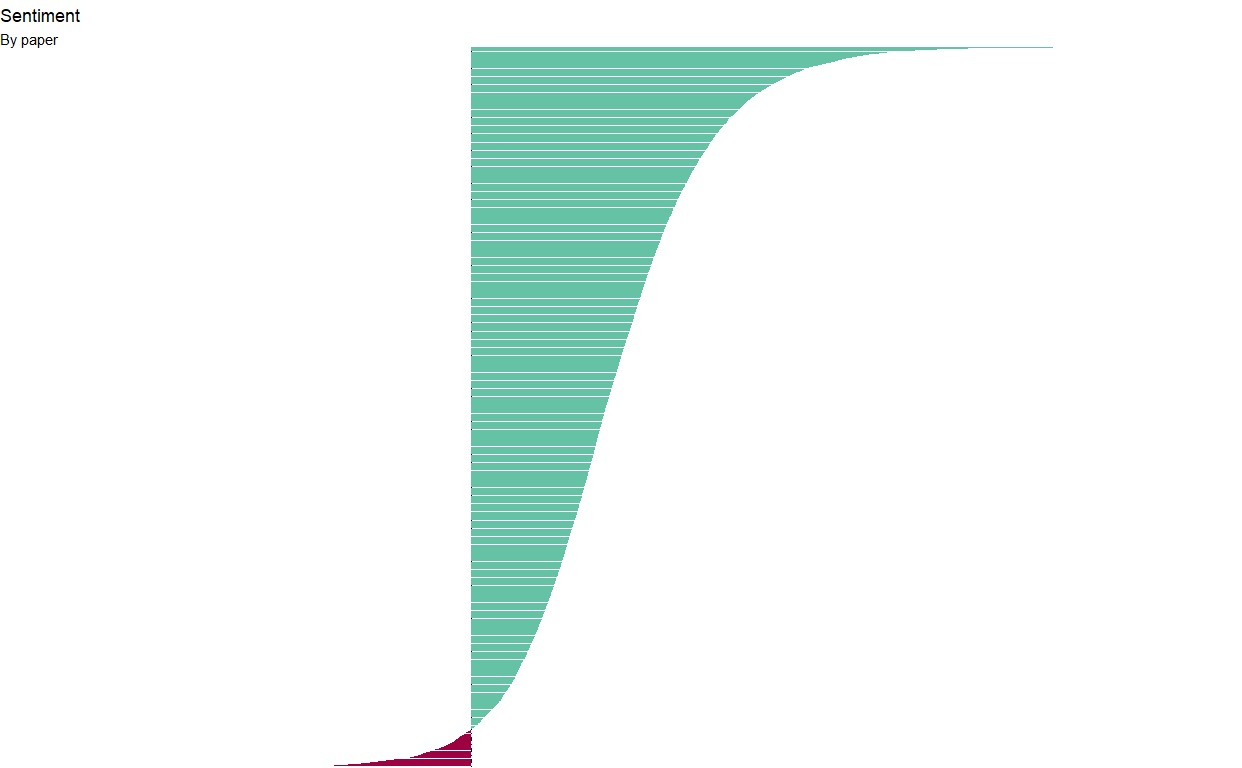
\includegraphics[width=4.6875in,height=\textheight]{images/sentimentPerPaper.jpg}

The above two graphs represent the average sentiment for each paper
based on its abstract. The first graph shows that most of the papers
have a positive sentiment of around 0,2. The send graphs shows that the
majority of the papers have a postie average sentiment, the negative
papers are a small proportion of the total.

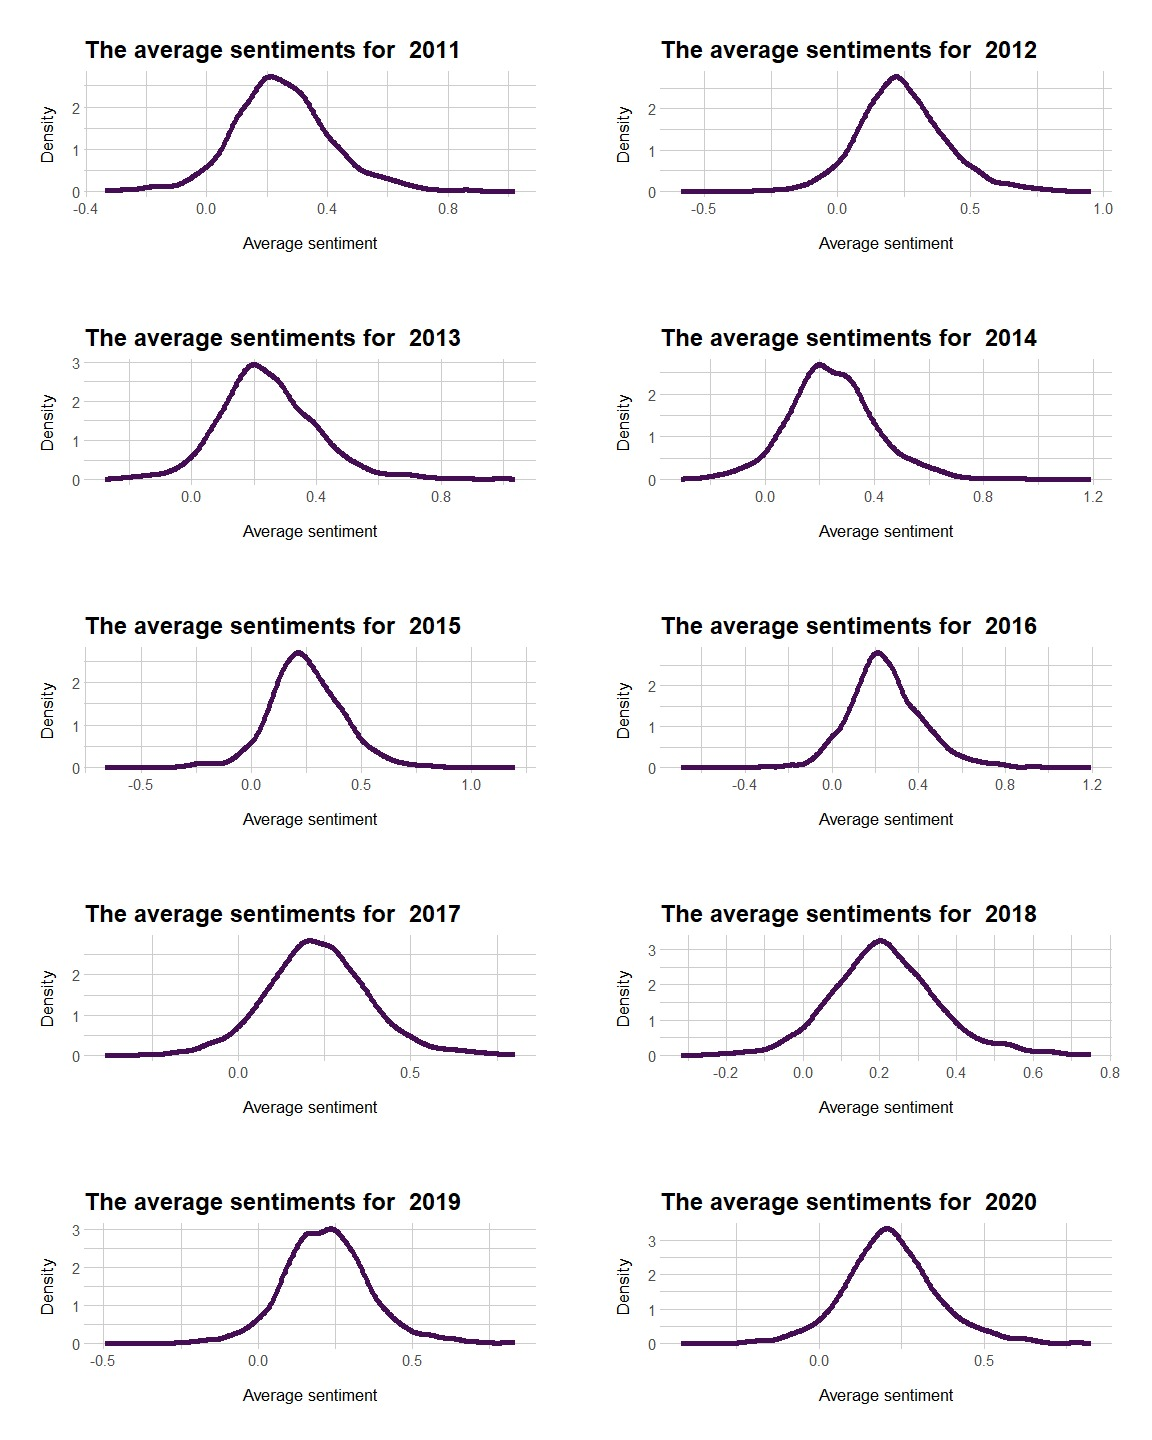
\includegraphics[width=5.20833in,height=\textheight]{images/aveSentimentPerYear.jpg}

The above graph shows any changes in tonality across abstracts for each
year. All the years differ slightly, but are all positive on average.

\hypertarget{average-per-topic}{%
\subsubsection{Average per topic}\label{average-per-topic}}

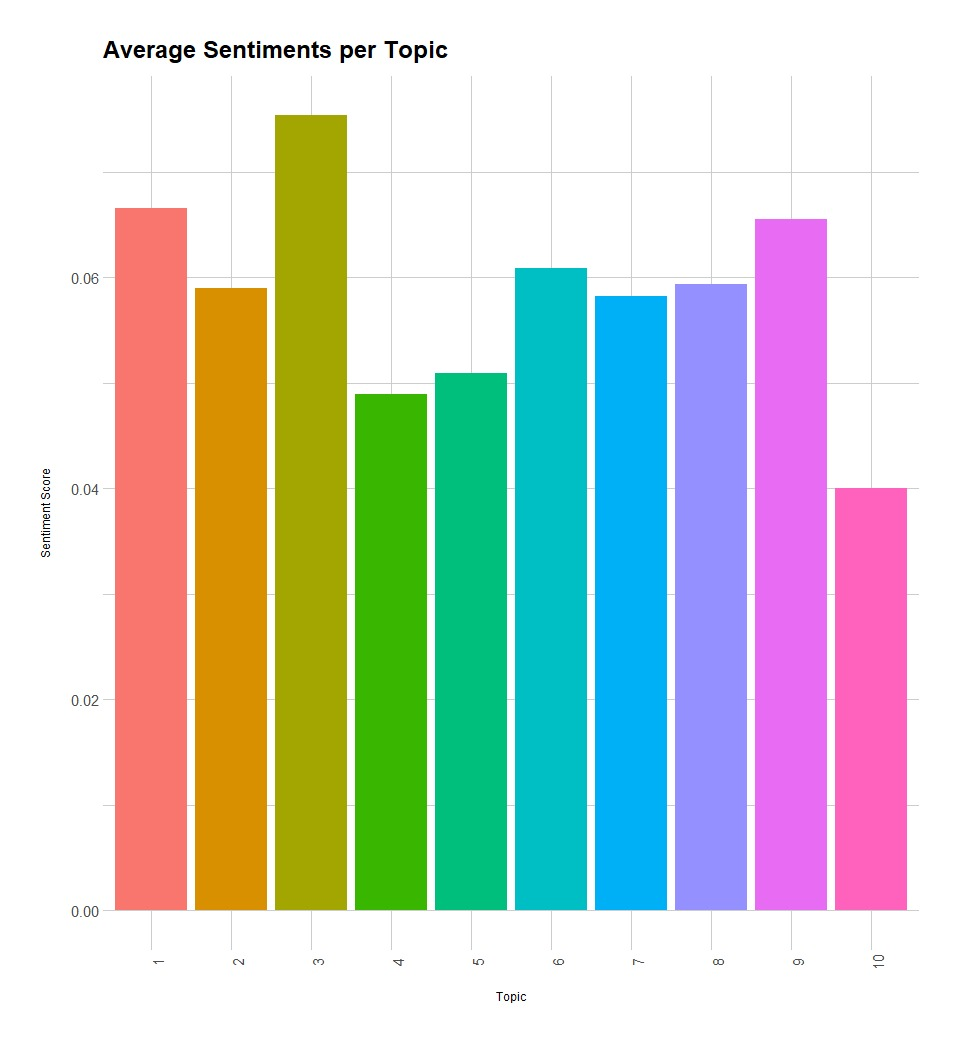
\includegraphics[width=5.20833in,height=\textheight]{images/aveSentimentPerTopic.jpg}

The above graph displays the average sentiment for each topic. This
metric is calculated using the beta for the terms of each topic as well
as the value of each term from the afinn sentiment database. This shows
that most topics are positive, with topic 3 being the most
positive.Topic 4 is the least positive of all.

\hypertarget{proportional-sentiments}{%
\subsubsection{Proportional sentiments}\label{proportional-sentiments}}

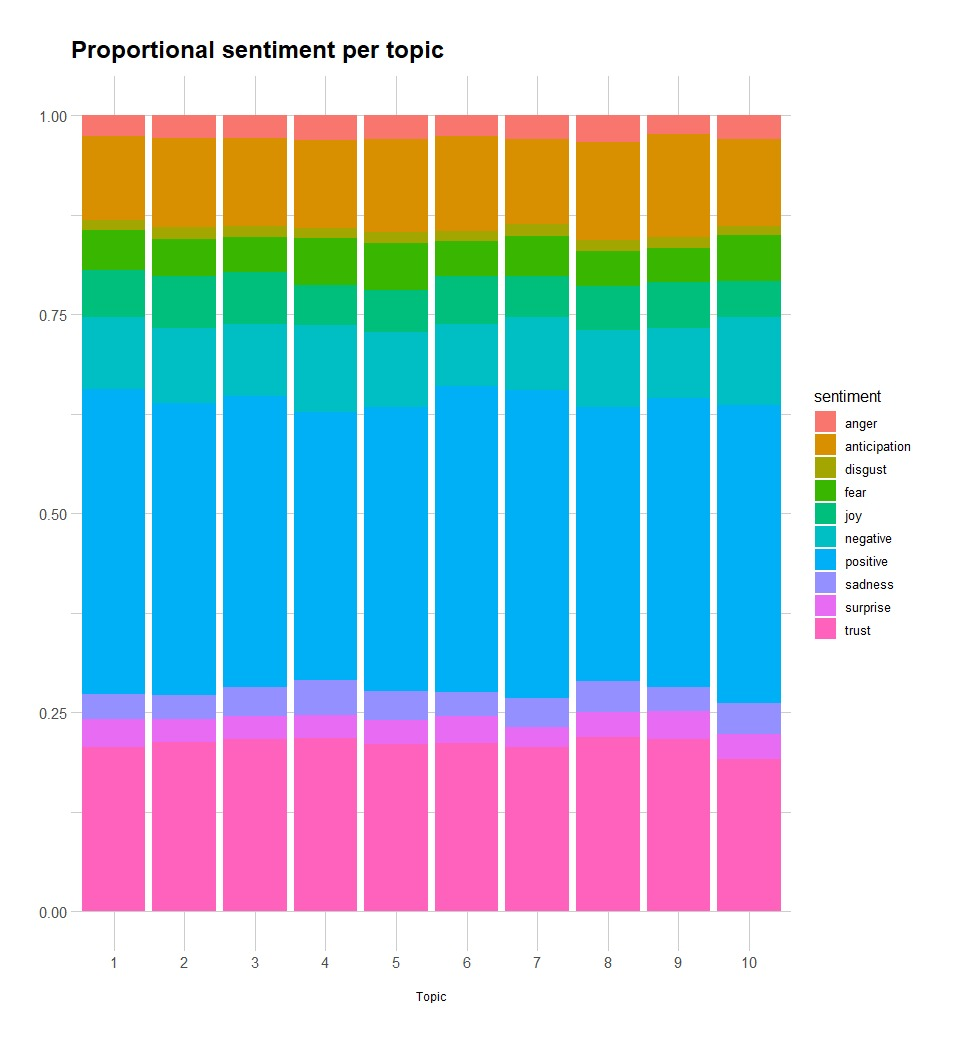
\includegraphics[width=5.20833in,height=\textheight]{images/PropSentimentPerTopic-01.jpg}

The above graph represents the portion that each sentiment category
takes up for each topic. Each topic has similar proportions for each
sentiment, with subtle differences in the postive and negative
sentiments. As shown, positive is the most prevalent sentiment,
contributing to most papers being positive on average.

\hypertarget{sentiments-per-topic}{%
\subsubsection{Sentiments per topic}\label{sentiments-per-topic}}

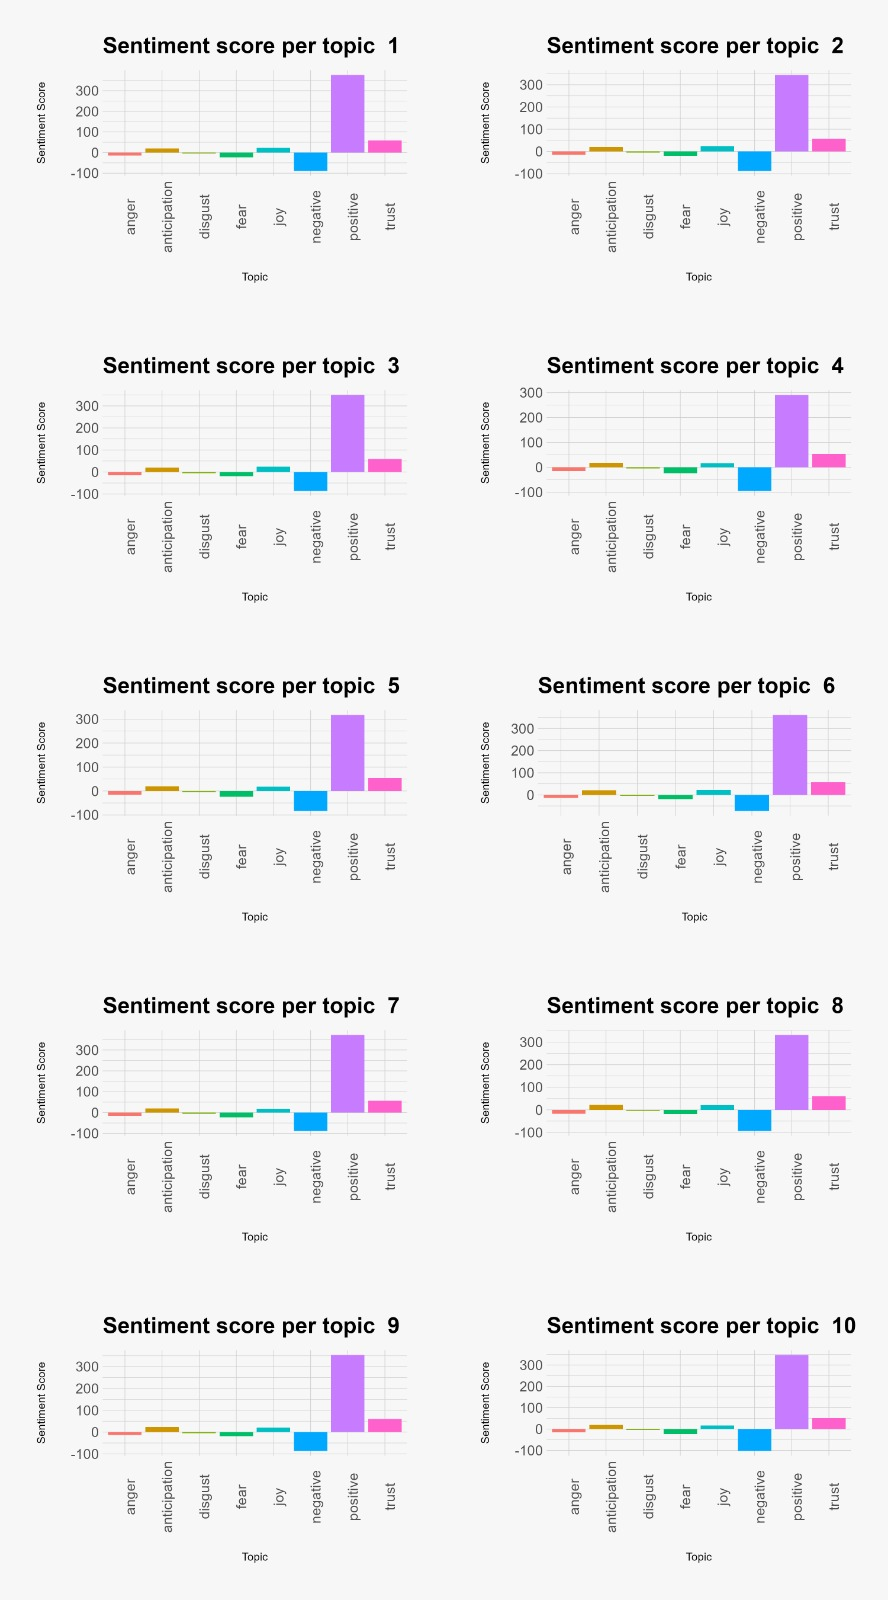
\includegraphics[width=5.20833in,height=\textheight]{images/SentimentScorePerTopic.jpg}

This above graph shows the sentiment proportions for each topic in more
detail. Each graph shows how much of each sentiment is in each topic,
with negative sentiments and emotions being negative on the y-axis.

\newpage{}

\hypertarget{conclusion}{%
\subsection{Conclusion}\label{conclusion}}

The field of Information Systems is a dynamic and evolving one. Through
this analysis of IS research from 2011 to 2020, we can see a shift in
themes and topics over the years. From research on traditional topics
such as knowledge management in the early 2010s to focusing more on
digital transformation and social media in later years. By investigating
the patterns in topics, authors, keywords and sentiments, we found the
field of Information Systems is adaptable and constantly evolving, and
researches technical issues as well as social issues.



\end{document}
